\chapter{The Response to Phenotypic Selection}
\marginnote{See \citet{lewontin1970units}. Note that these
  requirements are not specific to DNA, i.e. the concept of
  evolution by natural selection is substrate independent. }
Evolution by natural selection requires:
\begin{enumerate}
\item Variation in a phenotype
\item That survival is non-random with respect to this phenotypic
variation.
\item That this variation is heritable.
\end{enumerate}
Points 1 and 2 encapsulate our idea of Natural Selection, but evolution by natural
selection will only occur if the 3rd condition is also
met. \sidenote{Some people consider natural selection to only operate on heritable phenotype varation
  and so require all three conditions to say that natural selection
  occurs. This is mostly a semantic point, however, it is useful to be
able to distinguish the action of selection from a possible response.} It is the
heritable nature of variation that couples change within a generation
due to natural selection to change across generations (evolutionary
change). \\

Let's start by thinking about the change within a generation due
to directional selection, where selection acts to change the mean
phenotype within a generation. For example, a decrease in mean height within a
generation, due to taller organisms having a lower chance of surviving
to reproduction than shorter organisms. Specifically, we'll denote our mean phenotype at
reproduction by $\mu_S$, i.e. after selection has acted, and our mean
phenotype before selection acts by $\mu_{BS}$. This second quantity may be hard to
measure, as obviously selection acts throughout the life-cycle, so it
might be easier to think of this as the mean phenotype if selection
hadn't acted. So the change in mean phenotype within a generation is $\mu_{S} - \mu_{BS}= S$.  \\

\begin{marginfigure}
\begin{center}
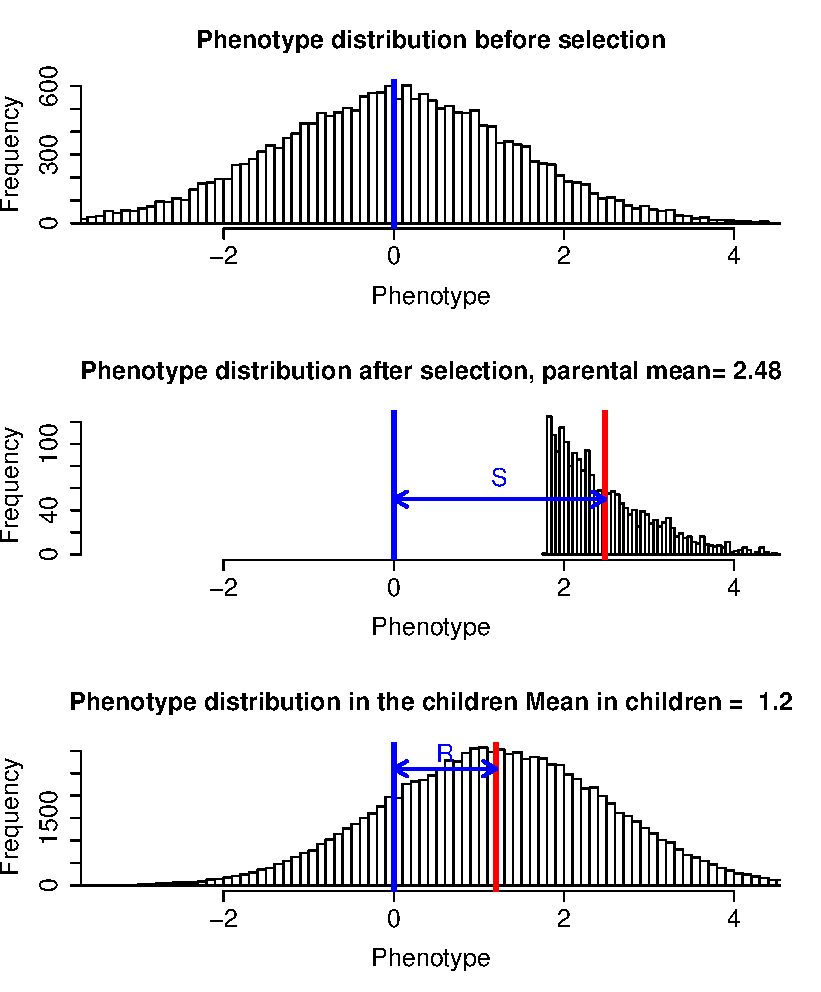
\includegraphics[width=\textwidth]{figures/Response_to_sel/QT3.pdf}
\end{center}
\caption{{\bf Top.} Distribution of a phenotype in the parental population
  prior to selection, $V_A=V_E=1$. {\bf Middle.} Only individuals in the top $10\%$
  of the phenotypic distribution are selected to reproduce; the resulting shift
  in the phenotypic mean is $S$. {\bf Bottom.}  Phenotypic distribution of
  children of the selected parents; the shift in the mean phenotype is
$R$. \gitcode{https://github.com/cooplab/popgen-notes/blob/master/Rcode/Quant_gen/QT3.R}}
\end{marginfigure}

We are interested in predicting the distribution of phenotypes in the next
generation. In particular, we are interested in the mean phenotype in
the next generation to understand how directional selection has
contributed to evolutionary change. We'll denote the mean phenotype in
offspring, i.e. the mean phenotype in the next generation before selection acts,
as $\mu_{NG}$. The change across generations we'll call the response
to selection $R$ and put this equal to $\mu_{NG}- \mu_{BS}$. \\


The mean phenotype in the next generation is
\begin{equation}
\mu_{NG} = \E \left( \E(X_{kid} | X_{mum},X_{dad}) \right)
\end{equation}
where the outer expectation is over possible pairs of randomly mating individuals
who survive to reproduce. We can use eqn. \ref{predict_kid} to obtain
an expression for this expectation:
\begin{equation}
\mu_{NG} = \mu_{BS} +
\beta_{mid,kid} ( \E(X_{mid}) - \mu_{BS})
\end{equation}

\begin{marginfigure}
\begin{center}
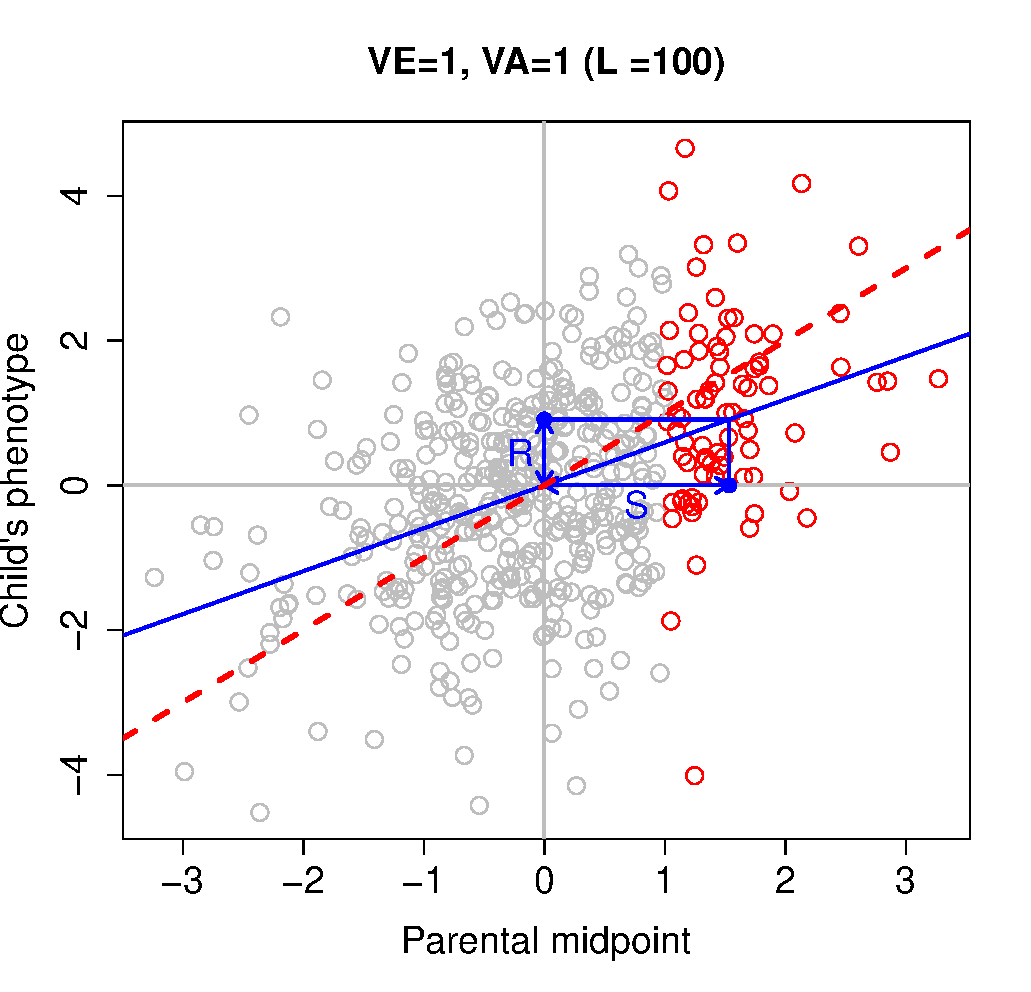
\includegraphics[width=\textwidth]{figures/Response_to_sel/Breeders_eqn.pdf}
\end{center}
\caption{A visual representation of the Breeder's equation. Regression
  of child's phenotype on parental mid-point phenotype
  ($V_A=V_E=1$). The parents and children of all families are shown as
  grey or red points, However, under truncation selection, only individuals
  with phenotypes $>1$ (red) are bred. The use of the red families
  only results in a phenotypic shift $S$ in the parental generation,
  which drives a shift $R$ in the offspring generation.
  \gitcode{https://github.com/cooplab/popgen-notes/blob/master/Rcode/Quant_gen/QT2.R}}
\end{marginfigure}

So to obtain $\mu_{NG}$ we need to compute $\E(X_{mid})$, the expected
mid-point phenotype of pairs of individuals who survive to
reproduce. Well this is just the expected phenotype in the individuals
who survived to reproduce ($\mu_{S}$), so
\begin{equation}
\mu_{NG} = \mu_{BS} +
h^2 (\mu_S - \mu_{BS})
\end{equation}
So we can write our response to selection as
\begin{equation}
R = \mu_{NG} -\mu_{BS}  =
h^2 (\mu_S - \mu_{BS}) = h^2 S \label{breeders_eqn}
\end{equation}
So our response to selection is proportional to our selection
differential, and the constant of proportionality is the narrow sense
heritability. This equation is sometimes termed the Breeder's
equation. It is a statement that the evolutionary change across
generations ($R$) is proportional to the change caused by directional selection
within a generation ($S$), and that the strength of this relationship is
determined by the narrow sense heritability ($h^2$). \\

%\graham{Lost the barncle question, put it back in.}



\begin{figure}
\begin{center}
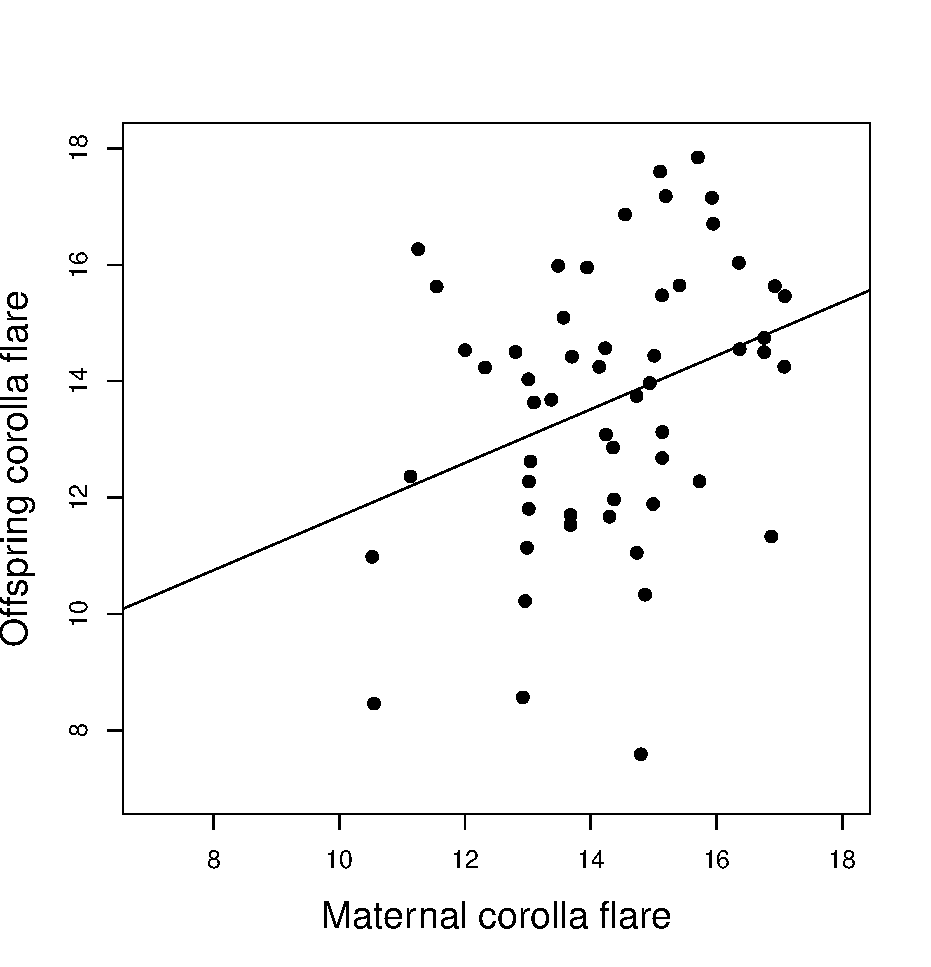
\includegraphics[width= 0.6 \textwidth]{Journal_figs/Quant_gen/Galen_flower_herit/Galen_corolla_flare.pdf} 
\end{center}
\caption{The relationship between maternal and offspring corolla flare (flower
  width) in P. viscosum. From \citeauthor{galen:96}'s data the
  covariance of mother and child is 1.3, while the variance of the
  mother is 2.8. Data from \citet{galen:96}. \gitcode{https://github.com/cooplab/popgen-notes/blob/master/Journal_figs/Quant_gen/Galen_flower_herit/Gallen_analysis.R}} \label{fig:Galen_corolla}  
\end{figure}

\begin{marginfigure}
\begin{center}
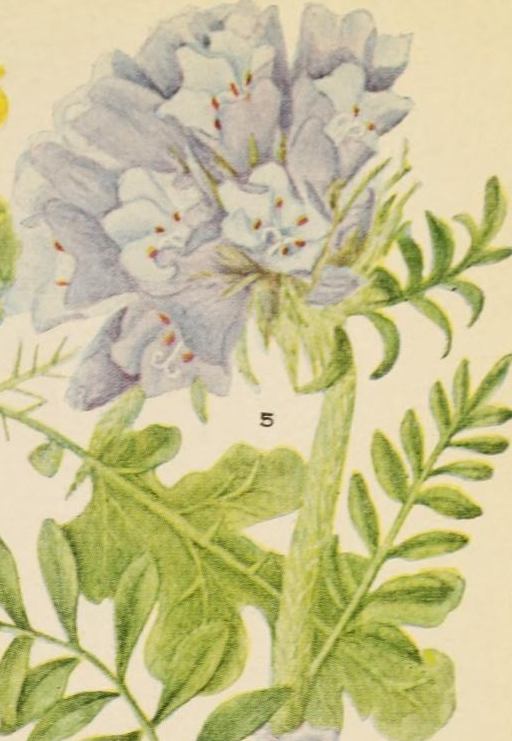
\includegraphics[width=0.75\textwidth]{illustration_images/Quant_gen/Polemonium_viscosum_Galen/Polemonium_viscosum.jpg}
\end{center}
\caption{Sticky jacob's ladder ({\it Polemonium viscosum}). \BHLNC{Flowers of Mountain and
    Plain (1920). Clements, E.}{https://www.biodiversitylibrary.org/page/40791993\#page/49/mode/1up}{New York Botanical Garden, Mertz Library}
Cropped from original.}
\end{marginfigure}


\begin{question}
\citet{galen:96} explored selection on flower shape in
{\it Polemonium viscosum}.  She found that plants with larger corolla flare
had more bumblebee visits, which resulted in higher seed set and a
$17\%$ increase in corolla flare in the plants contributing to the
next generation. Based on the data in the caption of Figure \ref{fig:Galen_corolla}
what is the expected response in the next generation?
\end{question}

\begin{marginfigure}
\begin{center}
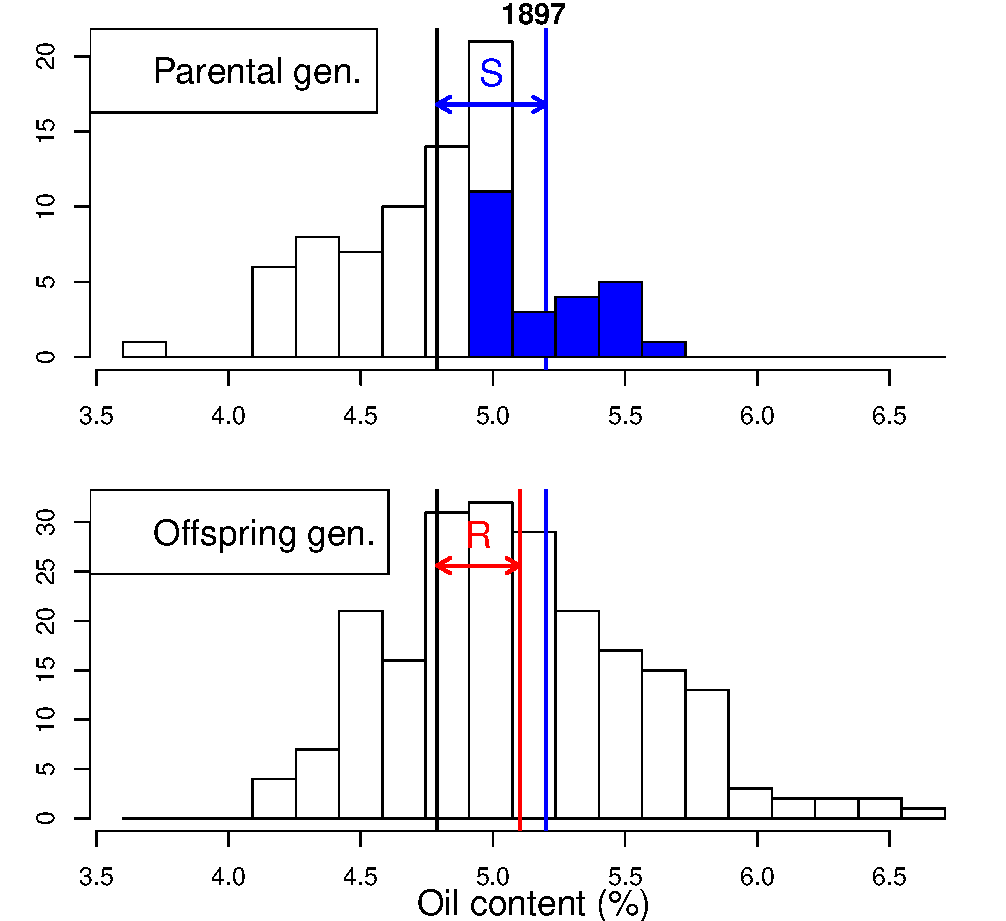
\includegraphics[width=\textwidth]{Journal_figs/Quant_gen/Illinois_long_term_selection_corn/Illinois_LTS_breeders_eq.pdf}
\end{center}
\caption{{\bf Top.} Phenotypic distribution of oil content in corn in
  1897, and the individuals who were selected to breed for the next
  generation are marked in blue.   {\bf Bottom.} The distribution in the next generation. Data from the
  Illinois selection experiment available \href{https://www.ideals.illinois.edu/handle/2142/3525}{here}, \gitcode{https://github.com/cooplab/popgen-notes/blob/master/Journal_figs/Quant_gen/Illinois_long_term_selection_corn/corn_LTS.R}}  \label{Illinois_LTS_breeders_eq}
\end{marginfigure}

If we know $R$ and $S$ we can estimate $h^2$. Heritabilities estimated
like this are called `realized heritability'. Estimates of the
`realized heritability' can readily be produced in artificial selection experiments:
\begin{question}
  From the experiment shown in Figure \ref{Fig:Illinois_LTS_breeders_eq},
  the mean corn oil content in 1897 was $4.78$, among the $24$ individuals
chosen to breed to for the next generation the mean was $5.2$. The
offspring of these individuals had a mean kernel oil content of
$5.1$. What is the narrow sense realized heritability? 
\end{question}

To understand the genetic basis of the response to selection take a
look at Figure \ref{Fig:Response_num_alleles}. The setup is the same as in our previous
simulation figures.
\begin{figure}
\begin{center}
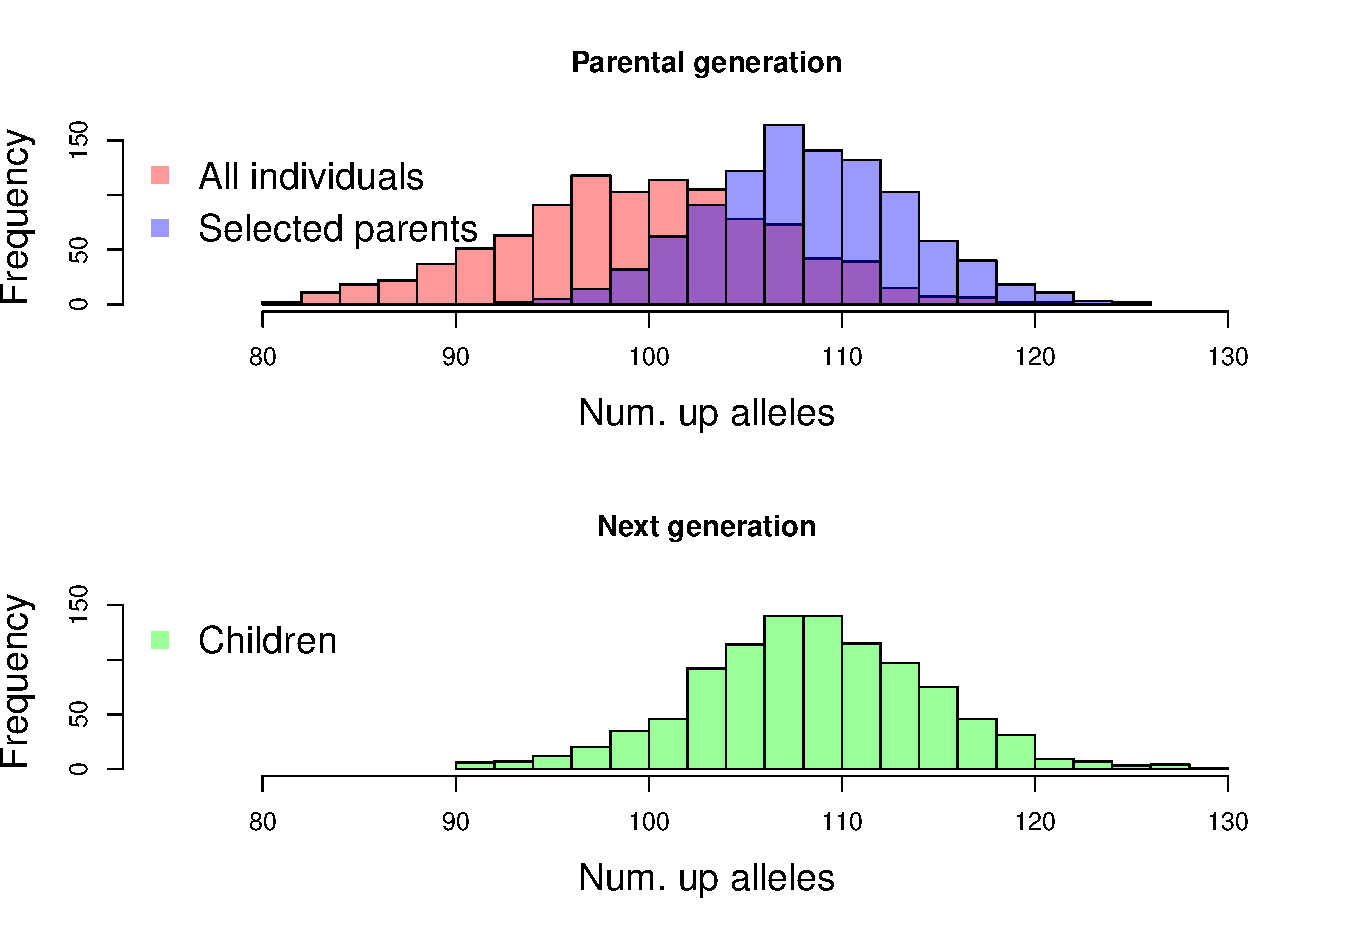
\includegraphics[width=\textwidth]{figures/QT3_w_genosums.pdf}
\end{center}
\caption[][4cm]{{\bf Top.} Distribution of the number of up alleles in the parental population
  prior to selection (red), for the selected individuals in the top
  $10\%$ phenotypic tail of the population (blue) {\bf Bottom.}  The same distribution
for the offspring of the selected parents in the next generation
(green). \gitcode{https://github.com/cooplab/popgen-notes/blob/master/Rcode/Quant_gen/QT3.R}}  \label{Fig:Response_num_alleles}
\end{figure}
 The individuals who are selected to form our next generation carry
 more alleles that increase the phenotype in the current range of
 environments currently experienced by the population. The average
 individual before selection carried 100 of these `up' alleles, while the average
 individual surviving selection carries 108 `up' alleles.
 \begin{marginfigure}[4cm]
 \begin{center}
   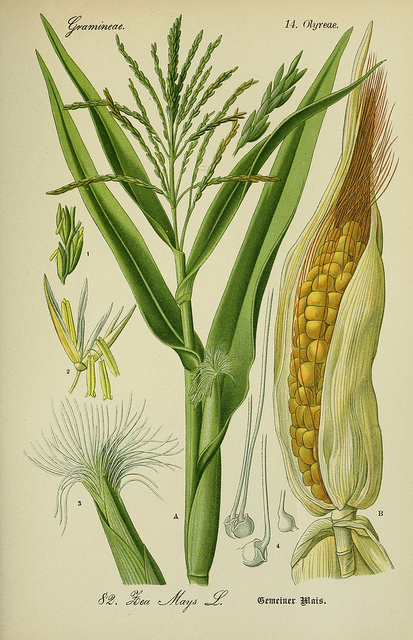
\includegraphics[width = 0.7 \textwidth]{illustration_images/Genetic_drift/maize/7845339168_66aa3d8ccc_z.jpg}
 \end{center}
 \caption{Maize ({\it Zea mays}.) \BHLNC{Prof. Dr. Thomé's Flora von
   Deutschland. 1886. Thomé, O. W.}{https://www.biodiversitylibrary.org/page/12306602\#page/669/mode/1up}{New York Botanical Garden}} \label{fig:maize}  %é
 \end{marginfigure}  %%possible different fig https://peerj.com/preprints/26502.pdf from Jeff's paper

 As individuals
 faithfully transmit their alleles to the next generation the average
 child of the selected parents carries 108 up alleles. Note that the
 variance has changed little, the children have plenty of variation in
 their genotype, such that selection can readily drive evolution in future generations. The average frequency of an `up' allele has changed
 from $50\%$ to $54\%$. Gains due to selection will be stably
 inherited to future generations and can be compounded on generation
 after generation if selection pressures were to remain constant.



 \subsection{The Long-Term Response to Selection}
   \begin{marginfigure}
 \begin{center}
 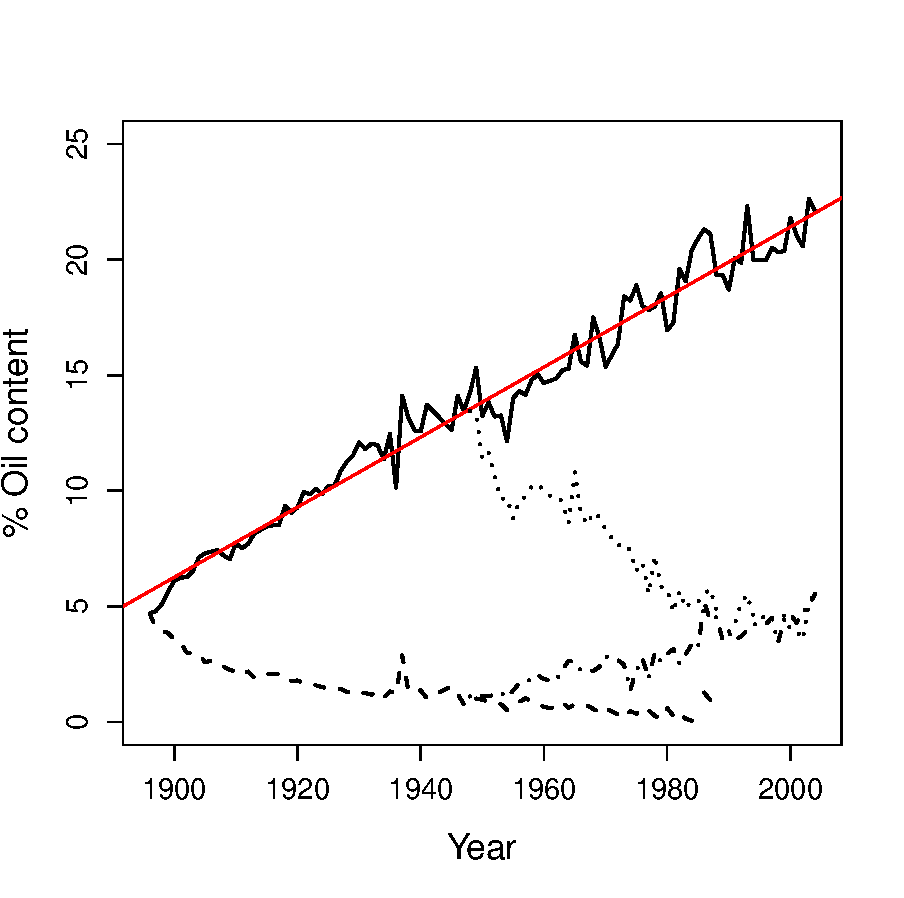
\includegraphics[width=\textwidth]{Journal_figs/Quant_gen/Illinois_long_term_selection_corn/Illinois_LTS_means.pdf} \end{center}
 \caption[2cm]{The mean oil content of corn in the Illinois long term
   selection experiment. Two populations were established in 1896 from
 the same inital population. Two secondary populations were
 established in 1948 where the direction of selection was reversed.
 Linear fit to the up experiment shown as a red line. Data available \href{https://www.ideals.illinois.edu/handle/2142/3525}{here}, \gitcode{https://github.com/cooplab/popgen-notes/blob/master/Journal_figs/Quant_gen/Illinois_long_term_selection_corn/corn_LTS.R}}\label{Fig:Illinois_LTS_means}
\end{marginfigure}

If our selection pressure is sustained over many generations, we can
use our breeder's equation to predict the response. If we are willing
to assume that our heritability does not change and we maintain a constant selection
differential ($S$), then after $n$ generations our phenotype mean will have
shifted 
\begin{equation}
n h^2 S
\end{equation}
i.e. our population will keep up a linear response to selection.
 \begin{figure}
 \begin{center}
   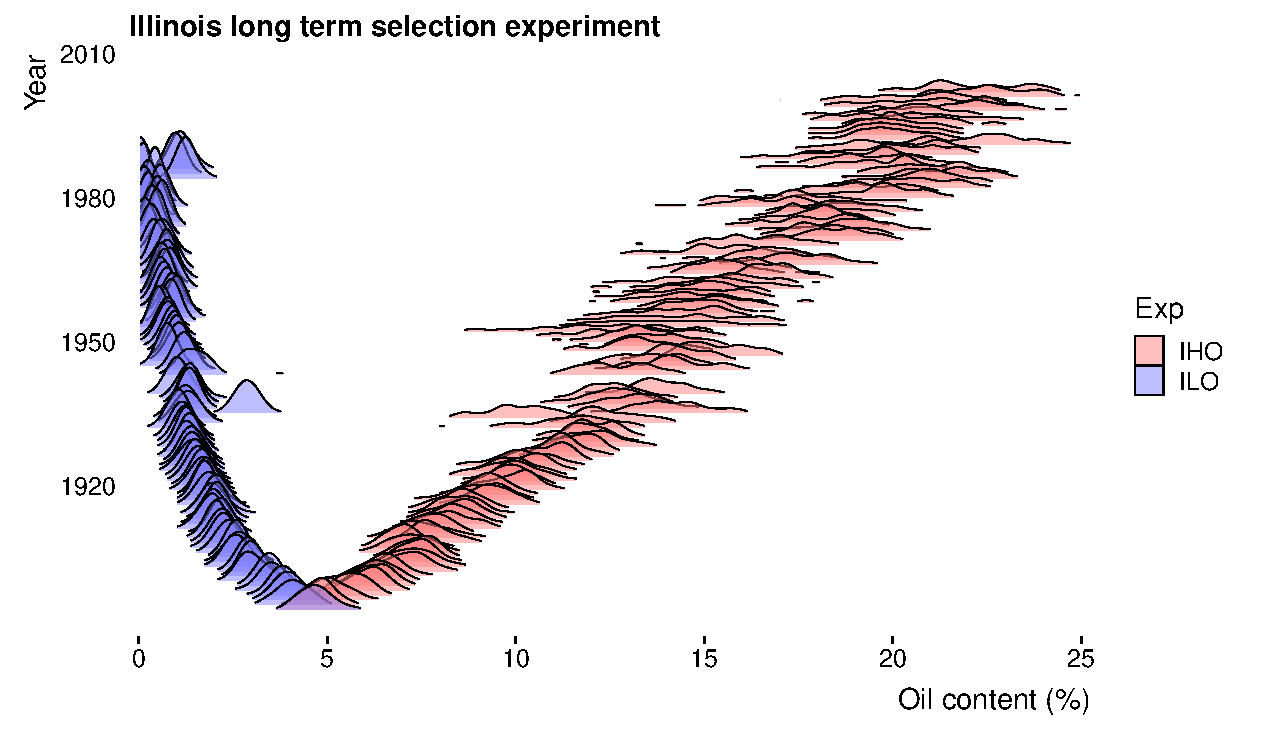
\includegraphics[width=\textwidth]{Journal_figs/Quant_gen/Illinois_long_term_selection_corn/Illinois_LTS_ggridges_distribution.pdf}\end{center}
 \caption[][5.5cm]{Density plots showing the phenotypic distributions of the
   up- and down-selection populations of the Illinois long term
   selection experiment over time. Data available
   \href{https://www.ideals.illinois.edu/handle/2142/3525}{here}, \gitcode{https://github.com/cooplab/popgen-notes/blob/master/Journal_figs/Quant_gen/Illinois_long_term_selection_corn/corn_LTS.R}}\label{Fig:Illinois_LTS_dists}
 \end{figure}
Therefore, long-term, consistent selection can drive impressive
evolutionary change. One example of this comes from a field experiment
in Illinois, where plant breeders have systematically selected for
higher and lower oil content in corn (see our previous Figure
\ref{Illinois_LTS_breeders_eq} for one generation of up selection). For over a century, they have taking seeds from the plants
in the extremes of the distribution and using them to form the next
generation. They have achieved impressive long-term responses, pushing
the population distributions well beyond their initial range (Figure \ref{Fig:Illinois_LTS_dists}.. They've established
two secondary populations where the selection differential was reversed. In the up-selection population they have maintained an
impressively linear increase in oil content, shown by red line in
Figure \ref{Fig:Illinois_LTS_means}, but while the
response is linear at first in the down line but they quickly reach
very low oil content.

%%single episide of selection in cliff swallows https://www.jstor.org/stable/2411315?mag=driving-evolution-cliff-swallows&seq=1#metadata_info_tab_contents
% http://mooselab.cropsci.illinois.edu/longterm.html
% https://www.ideals.illinois.edu/handle/2142/3525


\begin{question} \label{question:red_deer}
A population of red deer were trapped on Jersey (an island off of
England) during the last inter-glacial period. From the fossil record \cite{lister:89}
we can see that the population rapidly adapted to their new
conditions, perhaps due to selection for shorter reproductive times in
the absence of predation. Within 6,000 years they evolved from an estimated mean weight of
the population of 200kg to an estimated mean weight of 36kg (a 6 fold
reduction)! You estimate that the generation time
of red deer is 5 years and, from a current day population, that the narrow sense heritability of the
phenotype is 0.5.\\

 \begin{marginfigure}
 \begin{center}
 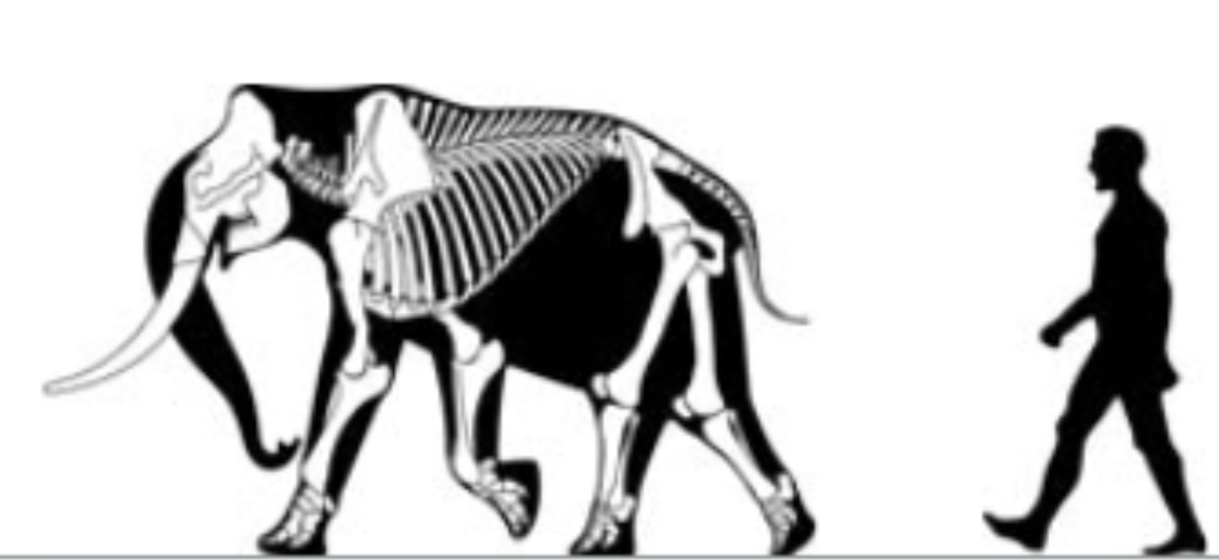
\includegraphics[width=\textwidth]{illustration_images/Quant_gen/dwarf_elephant/M_exilis_skeletal.pdf} \end{center}
 \caption{It's not just deer that evolve to be small on islands,
  pygmy mammoths and elephants have evolved from large mainland species
  on numerous islands. For example, the
   California Channel Islands were home to a dwarf mammoth until about 13,000 years
   ago. \newline \noindent \tiny{Santa
   Rosa {\it Mammuthus exilis}. \href{https://en.wikipedia.org/wiki/Pygmy_mammoth\#/media/File:M._exilis_skeletal.png}{wikimedia}, CC BY 3.0.} }\label{Fig:Pygmy_mammoth}
 \end{marginfigure}
{\bf A)}	Estimate the mean change per generation in the mean body weight. \\

{\bf B)}	Estimate the change in mean body weight caused by
selection within a generation. State your assumptions.\\

{\bf C)}	Assuming we only have fossils from the founding population and the population after 6000 years, should we assume that the calculations accurately reflect what actually occurred within our population?
\end{question}


In wild populations, selection pressures are likely rarely sustained 
for large numbers of generations. For example, the Grants' have
measured phenotypic selection in Darwin's Finches over multiple
decades on the island of Daphne Major. They have seen that
selection pressures in the Medium ground-finch ({\it Geospiza fortis})
have reversed a number of times over the years (Figure
\ref{fig:Darwins_Finches_unpred}). 
\graham{change to selection diff}
\begin{figure}
\begin{center}
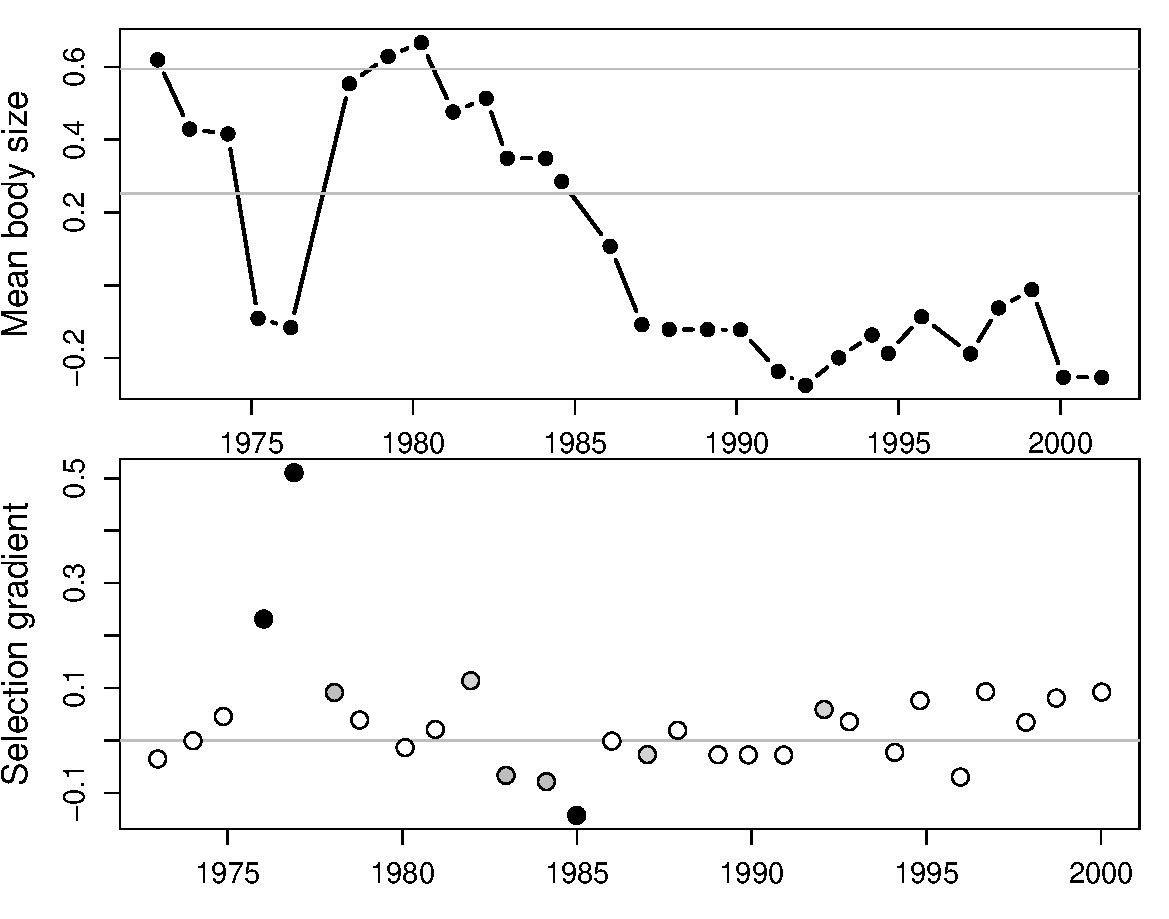
\includegraphics[width= 0.8 \textwidth]{Journal_figs/Quant_gen/Darwins_Finches_unpred/Darwins_Finches_unpred.pdf}
\end{center}
\caption[4cm]{{\bf Top)} Mean body size of the Medium ground-finch
  population measured each year. The 1973 $95\%$ confidence intervals
  are shown as horizontal bars. {\bf Bottom)} Standardized
  selection differentials on body size. The statistical significance of
  the selection differentials is shown, black points are $p<0.001$ and grey $p<0.05$.
  Data from \citet{grant2002unpredictable} \gitcode{https://github.com/cooplab/popgen-notes/blob/master/Journal_figs/Quant_gen/Darwins_Finches_unpred/Darwins_Finches_unpred.R}} \label{fig:Darwins_Finches_unpred}  
\end{figure}

\begin{marginfigure}[1cm]
\begin{center}
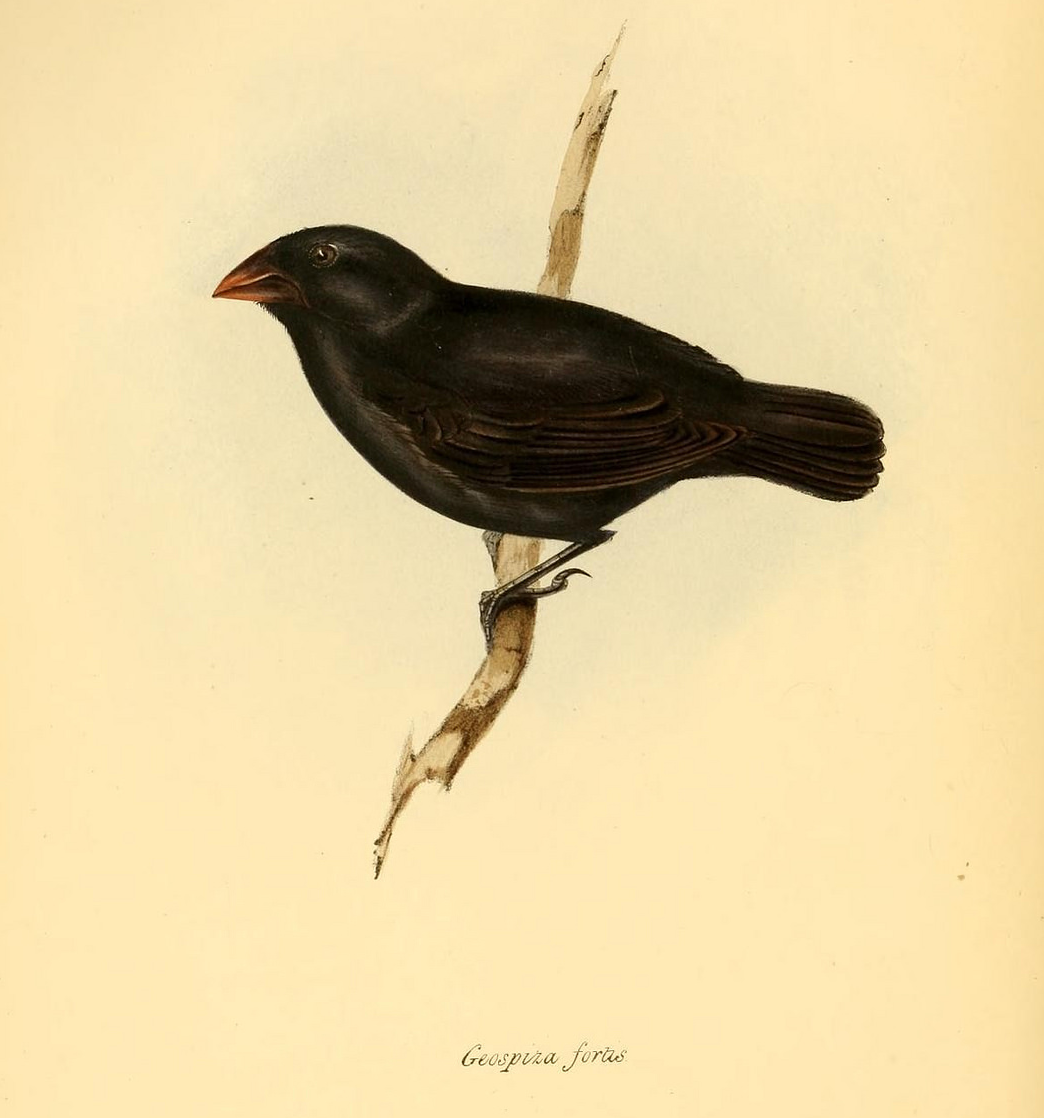
\includegraphics[width= \textwidth]{illustration_images/Quant_gen/Darwins_Finch/Geospiza_fortis.png}
\end{center}
\caption{Medium ground-finch ({\it Geospiza fortis}). \BHLNC{The zoology of
  the voyage of H.M.S. Beagle. Birds Part 3. (1841) Gould G. Edited by
  Darwin, C. Illustration by Elizabeth Gould.}{https://www.flickr.com/photos/biodivlibrary/8429528265/in/album-72157632647903291/}{Natural History Museum Library, London
}} \label{fig:Geospiza_fortis}  
\end{marginfigure}
%% Gingrich style data https://datadryad.org/resource/doi:10.5061/dryad.1tn7123?show=full
%% https://datadryad.org/resource/doi:10.5061/dryad.7d580


\paragraph{Patterns of long-term phenotypic change in the wild.}
Looking across the diversity of plants and animals we see huge changes
in size and form, can the strengths of selection we can observe over short time periods possibly explain
these changes?


To compare phenotypic changes over various time periods we need some measure of the rate of phenotypic
change. \citep{haldane1949suggestions} proposed the rate of change from
$X_1$ to $X_2$ in time interval $\Delta t$, measured in Millions of years, be quantified as
\begin{equation}
\frac{\log \left(\nicefrac{X_2}{X_1} \right) }{\Delta t}  = \frac{\log
  \left(X_2 \right) -\log \left(X_1 \right)  }{\Delta t} 
\end{equation}
by expressing this the log of the ratio\sidenote{Note that here, as
  elsewhere, $\log$ refers the natural logarithm, i.e. $\log$ base
  $e$. We'll make it clear if we using $\log$ in a different base,
  e.g. we'll use $\log_{10}$ for $\log$ in base 10.}, we are looking at the
proportional fold change, which makes sense as a
evolutionary change of 1cm in length is more impressive if you're a
mouse than an elephant. By putting this on a $\log$-scale we are
looking at the fold relative
change \citeauthor{haldane1949suggestions} called the
units of this measure {\emph`the Darwin'}, with a one Darwin change
corresponding to a $e\approx 2.71$
fold change in a Million years, a two Darwin change corresponding to a
$e^2\approx  7.34$ fold change in a Million years and so on. 

\begin{marginfigure}
  \begin{center}
    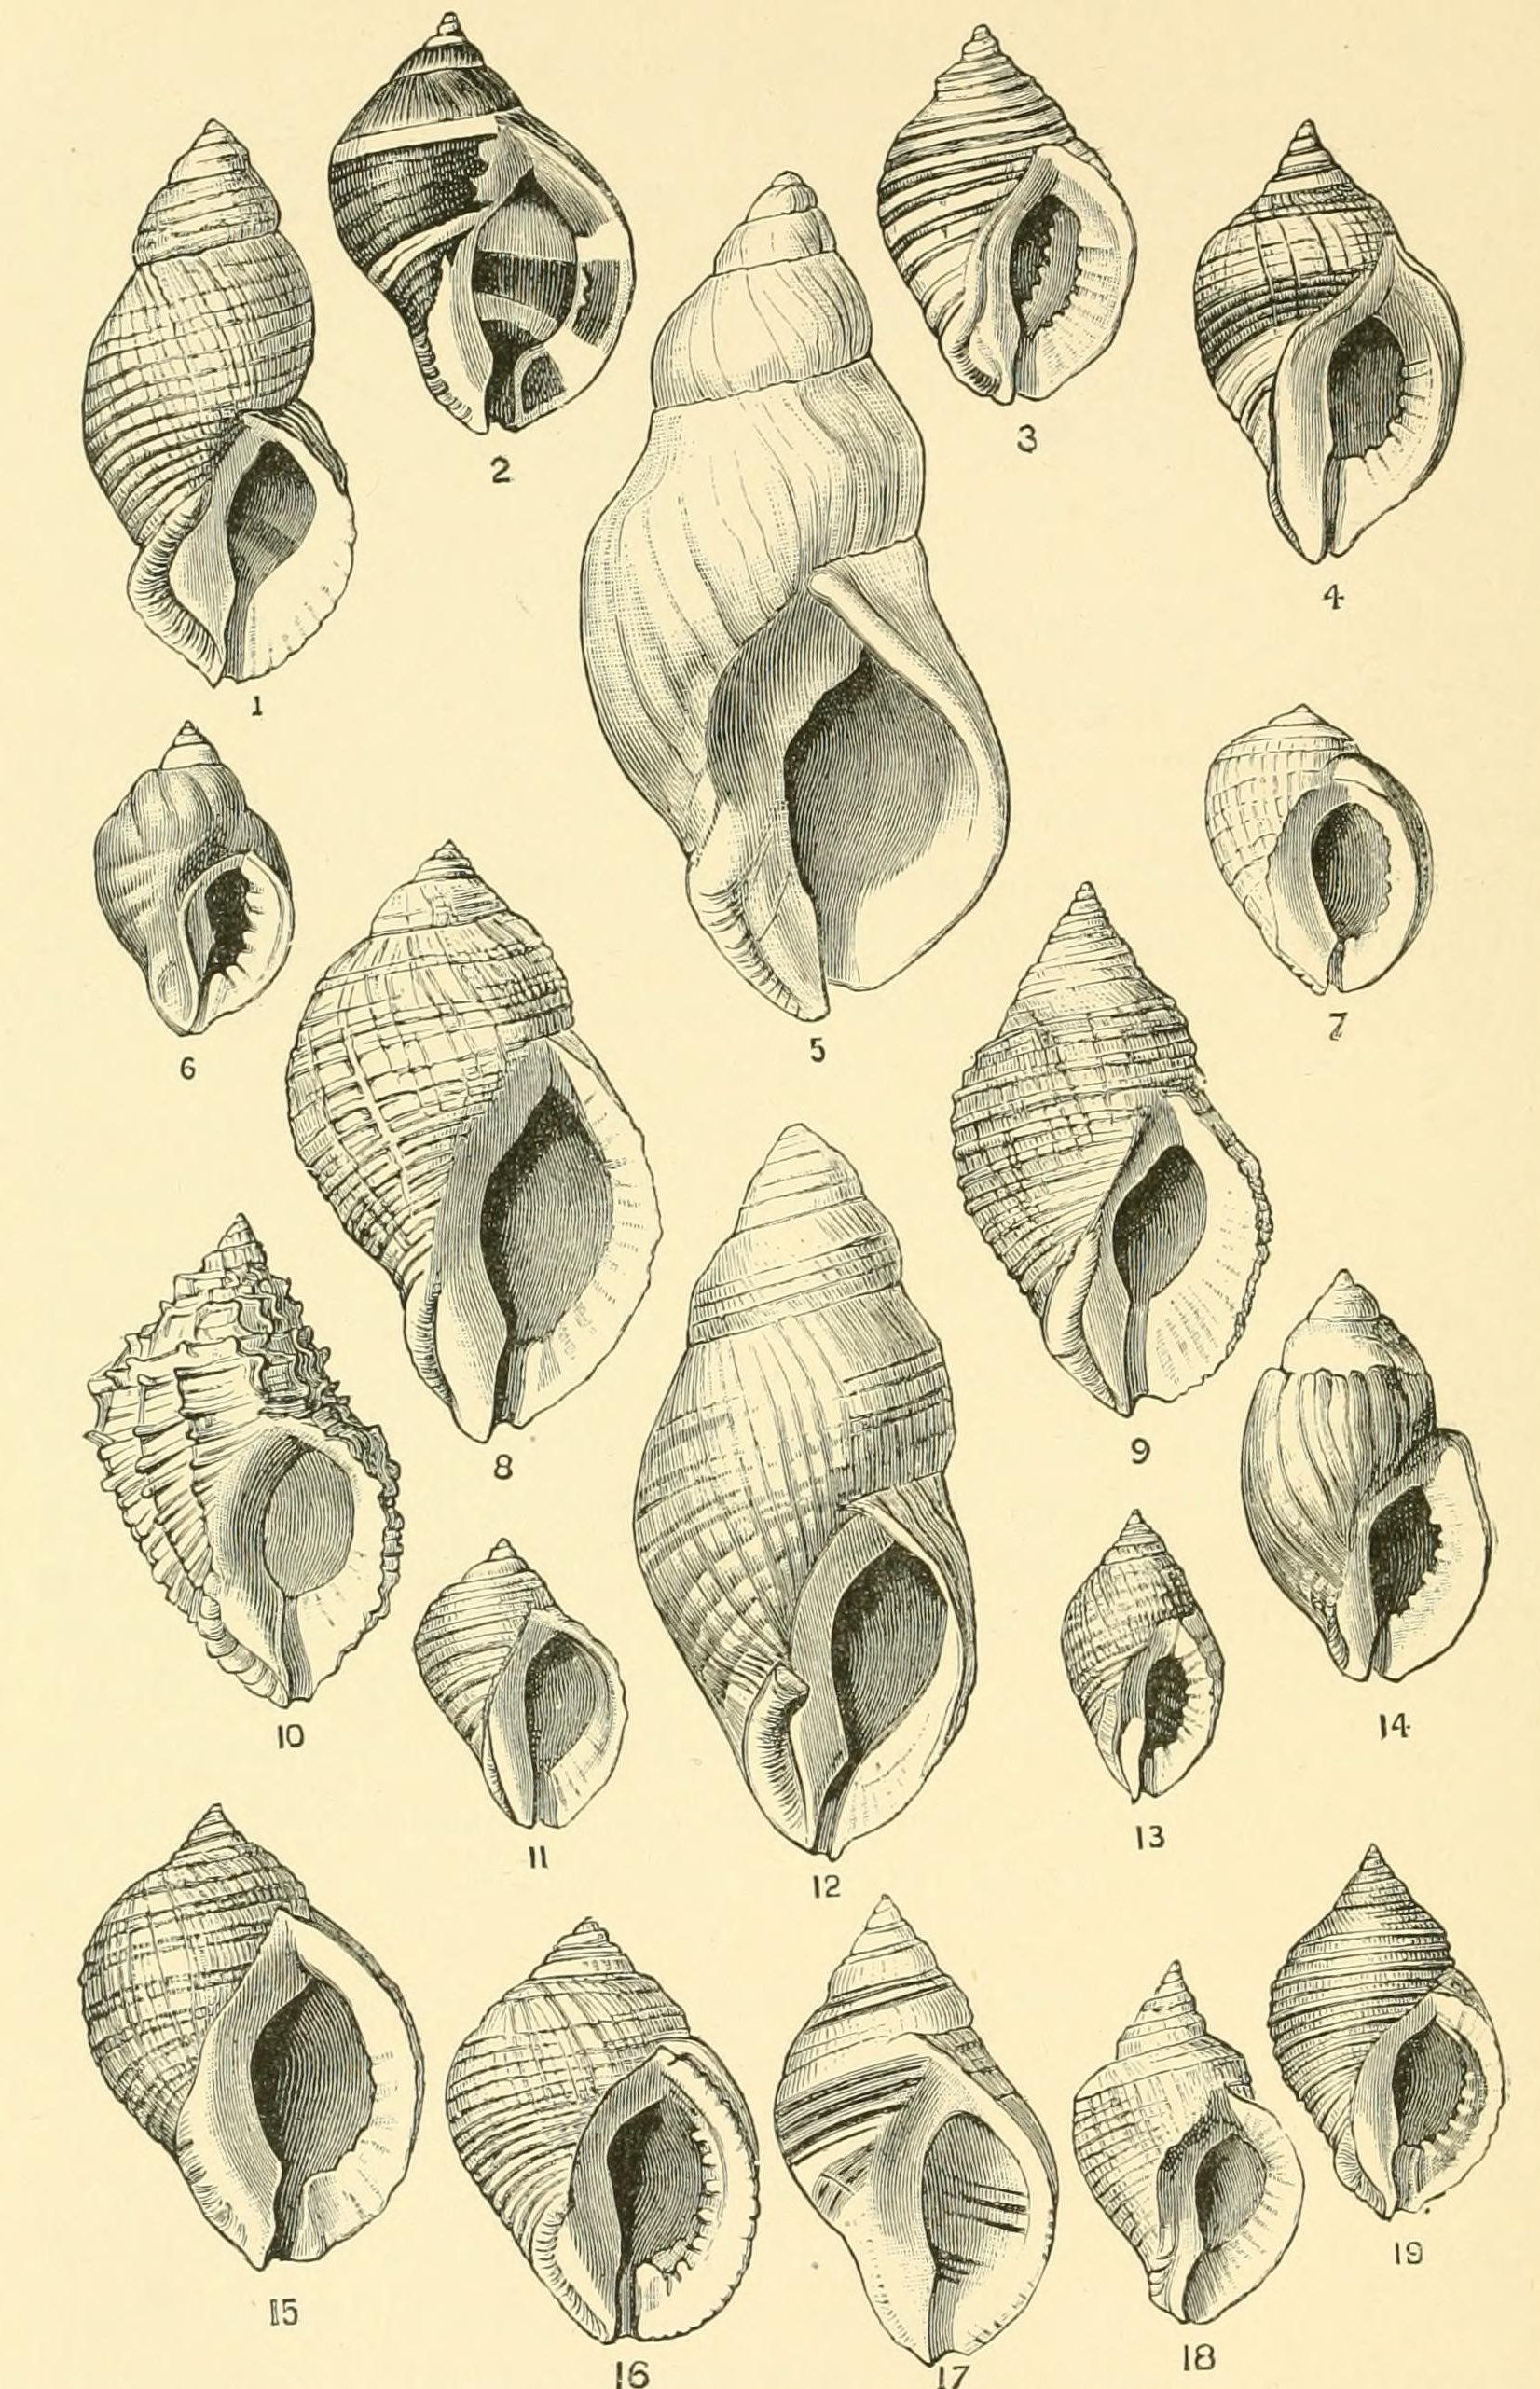
\includegraphics[width= \textwidth]{illustration_images/Quant_gen/dog_whelks/dog_whelks.jpg}
\end{center}
\caption{Variation in Atlantic dog whelks ({\it Nucella lapillus}, synonym {\it Purrpura lapukkus})
  along the coast of Great Britain.  \BHLNC{The Cambridge natural history, Molluscs and Brachiopods
    (1895). Cooke AH, Shipley AE, Reed FRC.}{https://archive.org/stream/cambridgenatural03har/cambridgenatural03har\#page/89/mode/1up}{University of Toronto - Earth Sciences Library}} \label{fig:dg_whelks}  
\end{marginfigure}


\begin{question}
Calculate the rate of change in body size in the Jersey red deer from
Question \ref{question:red_deer} in Darwins. Do the same for the total
change in corn oil content in the up lines in Figure \ref{Fig:Illinois_LTS_means}.
  \end{question}

\citet{gingerich1983rates} examined the absolute rate of phenotypic
change in field study data and the fossil record, a dataset
considerably expanded by \citet{uyeda2011million}. In Figure
\ref{fig:uyeda_gingerich} each point is an observation of phenotype
evolution. The x-axis shows the time period in years over which the
evolutionary change was observed, the x-axis is plotted on a
$\log_{10}$ scale.  The y-axis shows absolute rate of phenotypic
change, measured in Darwins, again on a $\log_{10}$, 

\begin{figure}
  \begin{center}
    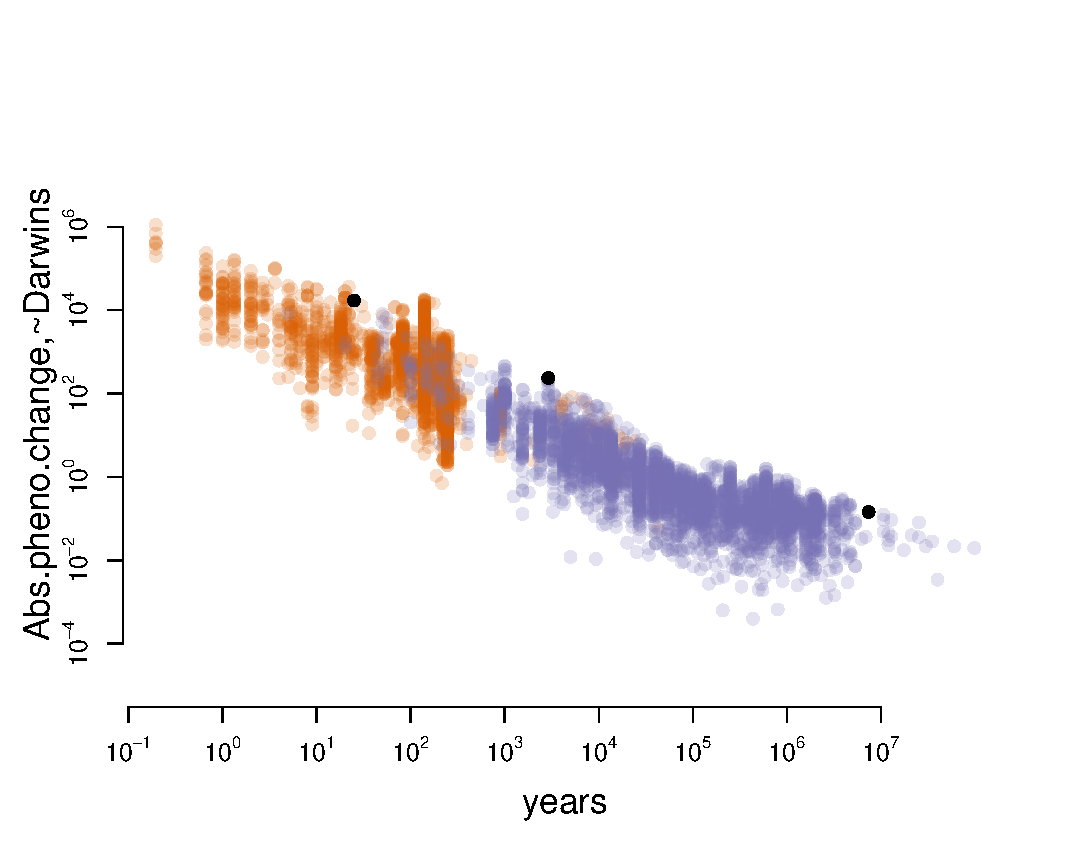
\includegraphics[width= \textwidth]{Journal_figs/Quant_gen/Uyeda_evol_rates/Uyeda_evol_rates.pdf}
\end{center}
\caption[][4cm]{The absolute rate of phenotypic evolution, measured in
  Darwins, plotted against the time interval over which the evolution
  was observed. The orange points show direct observations of
  phenotypic change in historical and contemporary populations. The
  blue dots give changes observed in the fossil record. The three
  black dots left to right give examples from Dog whelks, our Red deer example, and  {\it Triceratops}. Based on an original plot by
  \citet{gingerich1983rates} using an expanded dataset from
  \citet{uyeda2011million}. \gitcode{https://github.com/cooplab/popgen-notes/blob/master/Journal_figs/Quant_gen/Uyeda_evol_rates/Uyeda_evol_rates.R}} \label{fig:uyeda_gingerich}  
\end{figure}
Over short timescales we see incredibly rapid evolution, note the high
rates on the left of Figure \ref{fig:uyeda_gingerich}.
For example, the first black dot from the left is a case of evolution
over decades in dog whelks. The invasion the green crab ({\it Carcinus maenas})
drove the evolution of more robust shells in Atlantic dog
whelk ({\it Nucella lapillus}) in response to predation
along the North American coast \citep{vermeij1982phenotypic}. The shell lip thickness of dog whelks
in the St. Andrews, New Brunswick population had changed from 0.94mm
to 1.44mm in just 25 years. That's a 50\% increase, and a rate of
17060 Darwins.  \graham{is time interval wrong its 1920 to 1963 in
  Vermeij. }
\begin{marginfigure}
  \begin{center}
    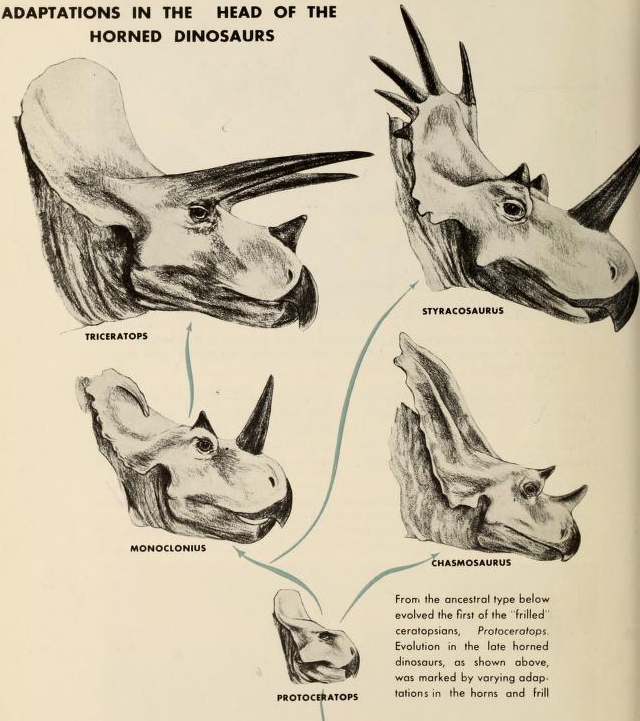
\includegraphics[width= \textwidth]{illustration_images/Quant_gen/Triceratops/Triceratops_phylo.png}
\end{center}
\caption{The evolution of {\it Triceratops} from {\it Protoceratops},
  see
  \href{https://www.geol.umd.edu/~tholtz/G104/lectures/104margino.html}{here}
  for a fun updated view of the {\it Coronosauria} phylogeny. See
  these
  \href{https://www.geol.umd.edu/~tholtz/G104/lectures/104margino.html}{figures}
  from Holtz for an updated \& fuller phylogeny. \IANC{The dinosaur book : the ruling reptiles and their
    relatives. (1951) Colbert, E.H.}{https://www.biodiversitylibrary.org/ia/bookruli00colb\#page/86/mode/1up}{American Museum of Natural History Library}} \label{fig:Triceratops_phyl}  
\end{marginfigure}
%% http://marsh.dinodb.com/marsh/Marsh%201891%20-%20Restoration%20of%20Triceratops%20(and%20Brontosaurus).pdf Marsh original pic of Triceratops
%https://www.geol.umd.edu/~tholtz/G104/lectures/104margino.html

However, when we observe phenotypic evolution over longer time periods
it is usually much
slower. For example, the rightmost black dot in Figure
\ref{fig:uyeda_gingerich} shows the phenotypic evolution along the
lineage leading to  {\it
  Triceratops}.   {\it Triceratops} measured in an impressive 25.9–29.5 ft in length. They evolved from a close
relative of {\it Protoceratops}, which was a bit bigger than a sheep
at $\sim$5.9 ft in about 7.5 million years
\citep{colbert1948evolution}. However, that's only a phenotypic change
of $0.143$ Darwins, its only a roughly four fold change in millions of
years. These rates of change in Dinosaurs have nothing on our dog
whelks, or many other examples of evolution on short time scales.    %https://www.geol.umd.edu/~tholtz/G104/lectures/104margino.html
Thus evolutionary changes we can observe over short timescales 
readily explain long term changes in quantitative phenotypes. 


\section{Fitness and the Breeder's Equation.}
So directional evolution occurs as selection drives a change in
the mean phenotype within a generation. But precisely how does this relate to
the natural-selection requirement that organisms vary in their
fitness? Some different ways of formulating the Breeder's equation
give us insight into the conditions for directional selection and the
relationship to fitness landscapes.

\subsection{Directional selection as the covariance between fitness and
phenotype.}
To think more carefully about this change within a
generation, let's think about a simple fitness model where our phenotype affects the
viability of our organisms (i.e. the probability they survive to
reproduce). The probability that an individual has a phenotype $X$
before selection is $p(X=x)$, so that the mean phenotype before
selection is
\begin{equation}
\mu_{BS} = \E[X] =  \int_{-\infty}^{\infty} x p(x) dx
\end{equation}
The probability that an organism with a phenotype $X$ survives to
reproduce is $w(X)$, and we'll think about this as the fitness of
our organism. The probability distribution of phenotypes in those who
do survive to reproduce is
\begin{equation}
\P(X | \textrm{survive}) =  \frac{p(x) w(x)}{
\int_{-\infty}^{\infty} p(x) w(x) dx}.
\end{equation}
where the denominator is a normalization constant which ensures that
our phenotypic distribution integrates to one. The denominator also
has the interpretation of being the mean fitness of the population,
which we'll call $\wbar$, i.e.  
\begin{equation}
\wbar =  \int_{-\infty}^{\infty} p(x) w(x) dx. \label{eqn:pheno_mean_fitness}
\end{equation}
Therefore, we can write the mean phenotype in those who survive to
reproduce as
\begin{equation}
\mu_S = \frac{1}{\wbar}\int_{-\infty}^{\infty} x p(x) w(x) dx
\end{equation}
\begin{marginfigure}
  \begin{center}
    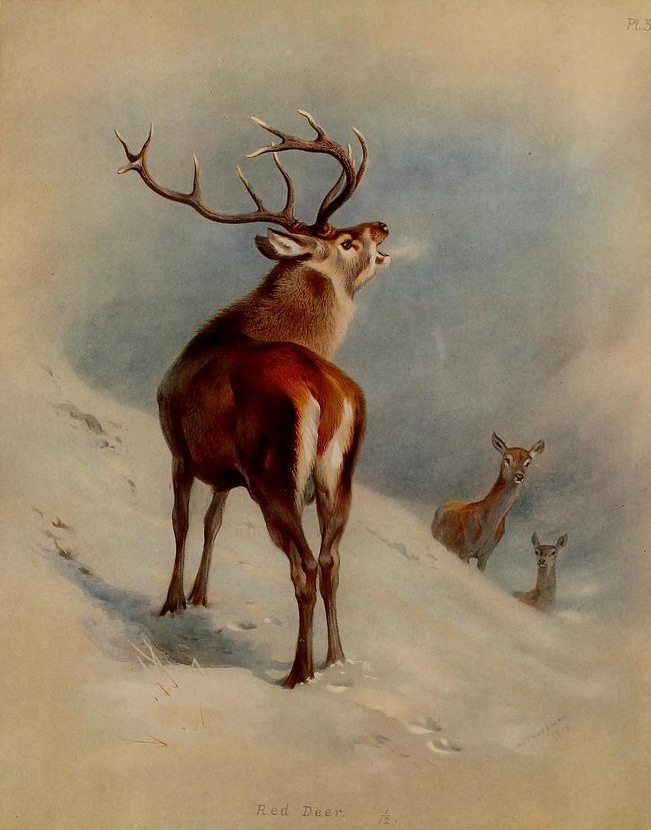
\includegraphics[width= \textwidth]{illustration_images/Quant_gen/red_deer/Red_deer.png}
\end{center}
\caption{Red deer ({\it Cervus elaphus}). \BHLCC{British
    mammals. Thorburn, A. (1920)}{https://www.flickr.com/photos/biodivlibrary/21269550204}{Field Museum of Natural History Library}{2.0}} \label{fig:red_deer}  
\end{marginfigure}

If we mean center the distribution of phenotypes in our population, i.e. set the phenotype before
selection to zero, then
\begin{equation}
S=\mu_S= \frac{1}{\wbar}\int_{-\infty}^{\infty} x p(x) w(x) dx = \frac{1}{\wbar}\E \left (X
  w(X) \right)
\end{equation}
% if $\mu_S=0$. \erin{do you mean $\mu_{BS}=0$?}
where the final part follows from the fact that the integral is taking
the mean of $X w(X)$ over the population.

As our phenotype is mean centered ($\E(X)=0$), we can see that $S$ has
the form of a covariance\sidenote{See our math appendix Equation \ref{eqn:def_covar} for the
definition of covariance.} between our phenotype $X$ and our relative fitness
$\nicefrac{w(X)}{\wbar} $. 
\begin{equation}
  S =  \E \left (X
  \nicefrac{w(X)}{\wbar} \right) =Cov \left(X, \nicefrac{w(X)}{\wbar} \right) \label{S_covar}
\end{equation}

  Thus our change in mean phenotype is directly a measure of the
  covariance of our phenotype and our fitness. 
  Rewriting our breeder's
equation using this observation we see
\begin{equation}
R = \frac{V_A}{V}  Cov \left(X, \nicefrac{w(X)}{\wbar} \right)  
\end{equation}

we see that the response to selection is due to the fact that our
fitness (viability) of our organisms/parents covaries with our phenotype, and
that our child's phenotype covaries with our parent's phenotype. 


\paragraph{Fitness Gradients and linear regressions}

To understand this in more detail let imagine that we calculate the
linear regression of an individual $i$'s mean-centered phenotype ($X_i$) on fitness ($W_i$), i.e. 
\begin{equation}
W_i \sim \beta X_i + \wbar \label{fitness_regression}
\end{equation}  
The best fitting slope of this regression ($\beta$), see math appendix
around eqn \ref{eqn:def_linear_regression} for more on linear regression, lets call it the
`fitness gradient', is given by
\begin{equation}
  \beta = Cov(X, \nicefrac{w(X)}{\wbar} )/ V  \label{beta_covar}
\end{equation}
\begin{marginfigure}[2cm]
\begin{center}
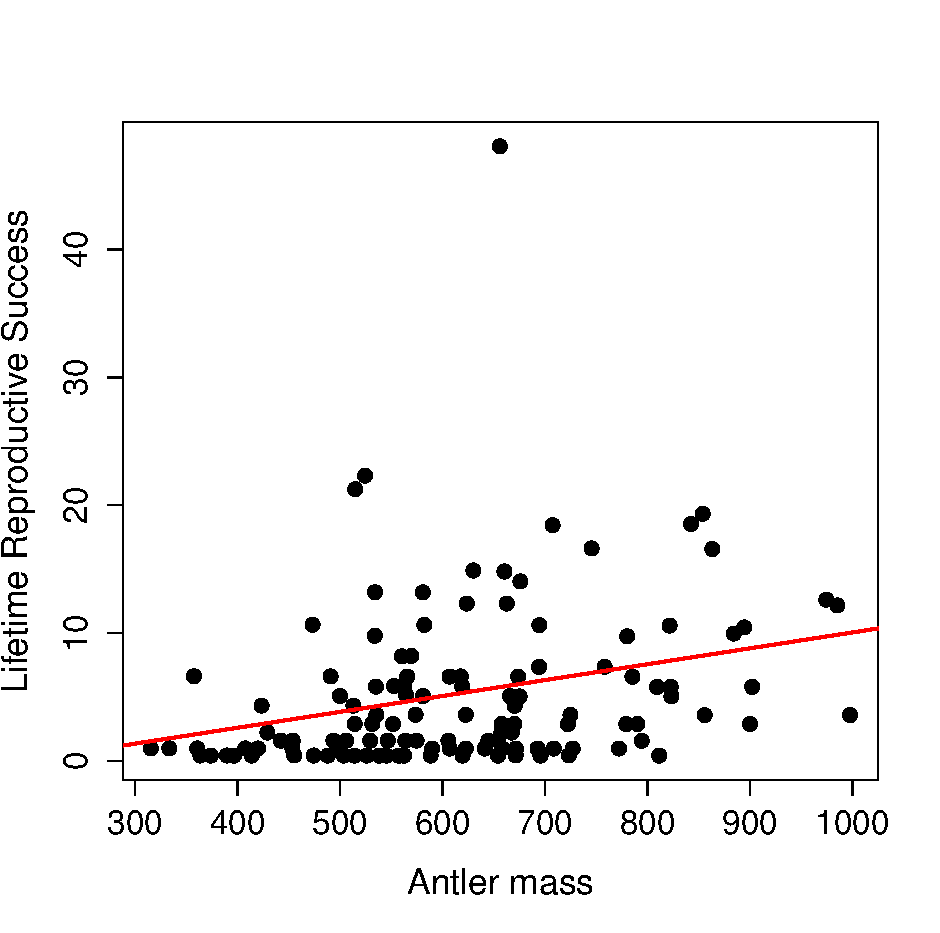
\includegraphics[width= \textwidth]{Journal_figs/Quant_gen/red_deer_selection_gradient/selection_grad_deer.pdf}
\end{center}
\caption{Lifetime reproductive success (LRS) of male Red Deer as a
  function of their antler mass. Data from \citet{kruuk2002antler};
  see the paper for discussion of the complexities of equating this
  selection gradient with the evolutionary response. \gitcode{https://github.com/cooplab/popgen-notes/blob/master/Journal_figs/Quant_gen/red_deer_selection_gradient/selection_grad_deer.R}. } \label{fig:red_deer_fitness_grad}  
\end{marginfigure}

  i.e. the fitness gradient is the phenotype-fitness
 covariance divided by the phenotypic variance. Using this result we can rewrite the breeder's equation as
\begin{equation}
R= V_A \beta \label{eqn:R_beta}
\end{equation}
i.e. we'll see a directional response to selection if there is a linear relationship of phenotype on fitness, and if there is additive genetic variance for the phenotype. As one example of a fitness gradient, in Figure \ref{fig:red_deer_fitness_grad}  the lifetime reproductive success (LRS) of male Red Deer is plotted against the weight of their antlers. The red line gives the linear regression of fitness (LRS) on antler mass and the slope of this line is the fitness gradient ($\beta$). 

\graham{add pic of relationship between slope and S?}

\paragraph{Fisher's fundamental theorem of natural selection} 
Finally how does the mean fitness of our population evolve? 
If we choose relative fitness to be our phenotype
  ($X=\nicefrac{w(X)}{\wbar}$), then the response in fitness is
\begin{align}
  R &= \frac{V_A}{V}  Cov \left(\nicefrac{w(X)}{\wbar} ,
  \nicefrac{w(X)}{\wbar} \right) = \frac{V_A}{V} V \nonumber\\
  &=V_A
\end{align}
i.e. the response to selection is equal to the additive genetic
variance for relative fitness. Or as Fisher put it
\begin{quote}
``The rate of increase in fitness of any organism at any time is equal
to its genetic variance in fitness at that time.'' -\citet{fisher1930} (pg 37)
\end{quote}
Fisher called this `the fundamental theorem of natural
selection'. Our proof here is just a sketch, and more formal
approaches are needed to show it in generality. There has been much gnashing of teeth over exactly how broadly this result holds, and exactly what
Fisher meant \citep[see ][ for a recent overview]{ewens2010gene}. 
% Ruth shaw FFTNS https://www.biorxiv.org/content/biorxiv/early/2019/04/07/601682.full.pdf
% https://commons.wikimedia.org/wiki/File:A_guide_to_the_wild_flowers_(Plate_CXXV)_BHL23798491.jpg

\subsection{Directional Selection on Fitness Landscapes.}  \label{section:pheno_fitness_landscapes}

 \begin{figure*}
 \begin{center}
 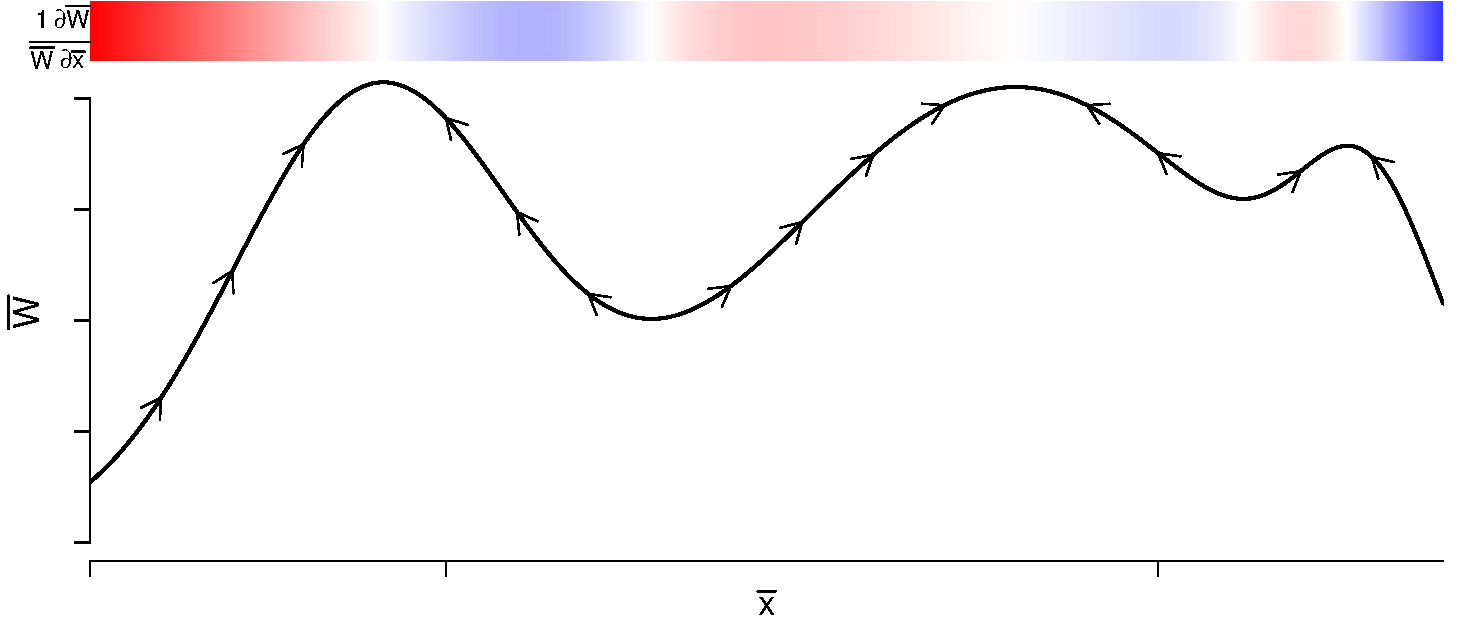
\includegraphics[width= 0.8 \textwidth]{figures/Response_to_sel/fitness_landscape_1D.pdf}
 \end{center}
 \caption{An example of a fitness landscape, showing the mean fitness
   of the population ($\wbar$) as a function of the mean phenotype of the
   population ($\bar{z}$, \gc{Need
   to change to $\bar{x}$}). The arrows show the expected direction of movement
of our population on the fitness landscape, with natural selection moving
our population toward local fitness optima. The coloured bar shows the
derivative (slope) of the mean fitness with respect to mean
phenotype (eqn. \eqref{eqn:pheno_fitness_landscape}). Red values are positive slopes corresponding to the population evolving
towards the right of the page, blue is a negative slope with the
population moving to the left. } \label{fig:fitness_landscape_1D}  
\end{figure*}

One common metaphor when we talk about evolution is that of a population exploring an adaptive landscape with natural selection pushing a population
towards higher fitness states corresponding to peaks in this landscape
(see e.g. Figure \ref{fig:fitness_landscape_1D}).  \graham{Simpson/Wright.}
\citet{lande1976natural} found an evocative formulation of the
Breeder's equation which aids our intuition of phenotypic fitness
landscapes. \graham{need note about when this breaks down}
\citeauthor{lande1976natural} showed that,
if the phenotype is
normally distributed, the response to
selection ($R$) could be written in terms of the gradient (derivative) of the
mean fitness ($\wbar$) of the population\sidenote[][-3cm]{
  This follows from the fact that we can then move the
  derivative inside the integral of $\wbar$, eqn \eqref{eqn:pheno_mean_fitness}, %$\nicefrac{\partial \log\wbar}{\partial \bar{x}} = \nicefrac{1}{\wbar} \nicefrac{\partial\wbar}{\partial \bar{x}}$.
to write the new term in eqn \eqref{eqn:pheno_fitness_landscape} as 
  \begin{align}
\frac{1}{\wbar}  \frac{\partial \wbar}{\partial \bar{x}} &=
                                                                   \frac{1}{\wbar}
                                                                   \int_{-\infty}^{\infty}w(x)
                               \frac{\partial p(x)}{\partial \bar{x}}  dx \nonumber\\
& =\int_{-\infty}^{\infty} \frac{w(x)}{\wbar}  \frac{(x-\bar{x})}{V}  dx  \nonumber\\
                             & = \frac{cov(w(x),x) }{var(x)} \label{eqn:proof_landscape}
\end{align}
which is $\beta$, so that eqns \eqref{eqn:R_beta} and
\eqref{eqn:pheno_fitness_landscape} are equivalent. For this equivalence
to hold, in the first line we assume that $w(x)$ is not a function
of $\bar{x}$, while the middle line is true when $p(x)$ is the normal distribution.
}
as a function of the mean phenotype:  
\begin{equation}
  R = \frac{V_A}{\wbar} \frac{\partial \wbar}{\partial \bar{x}}  \label{eqn:pheno_fitness_landscape}  %V_A 
 % \frac{\partial \log \left(\wbar \right)}{\partial \bar{z}}
\end{equation}

What does this mean? Well $\nicefrac{V_A}{\wbar}$ is always positive,
so the direction our population responds to selection is
predicted by the sign of the derivative (see Appendix Section
\ref{section:calculus} for more on derivatives). If increasing the mean
phenotype of the population slightly would 
increase mean fitness ($ \nicefrac{\partial \wbar}{\partial \bar{x}}
>0$) our population will respond that generation by evolving toward
higher values of the trait ($R>0$), left panel of Figure \ref{fig:fitness_landscape_1D_w_wbar}. Conversely, if decreasing the
population mean phenotype slightly would increase the mean fitness ($ \nicefrac{\partial \wbar}{\partial \bar{x}}
<0$) the population will that generation evolve towards lower values
of the phenotype  (middle panel of Figure
\ref{fig:fitness_landscape_1D_w_wbar}). Thus, if selection pressures
remain constant, we can think of the population as evolving on
an adaptive landscape where the elevation is given by the population mean
fitness. Natural selection operates on the basis of individual-level
fitness, but as a result of this our population is increasing in its
average fitness, i.e. our population is becoming better adapted. We'll
discuss the caveats of this hill-climbing interpretation below.

 \begin{figure*}
 \begin{center}
 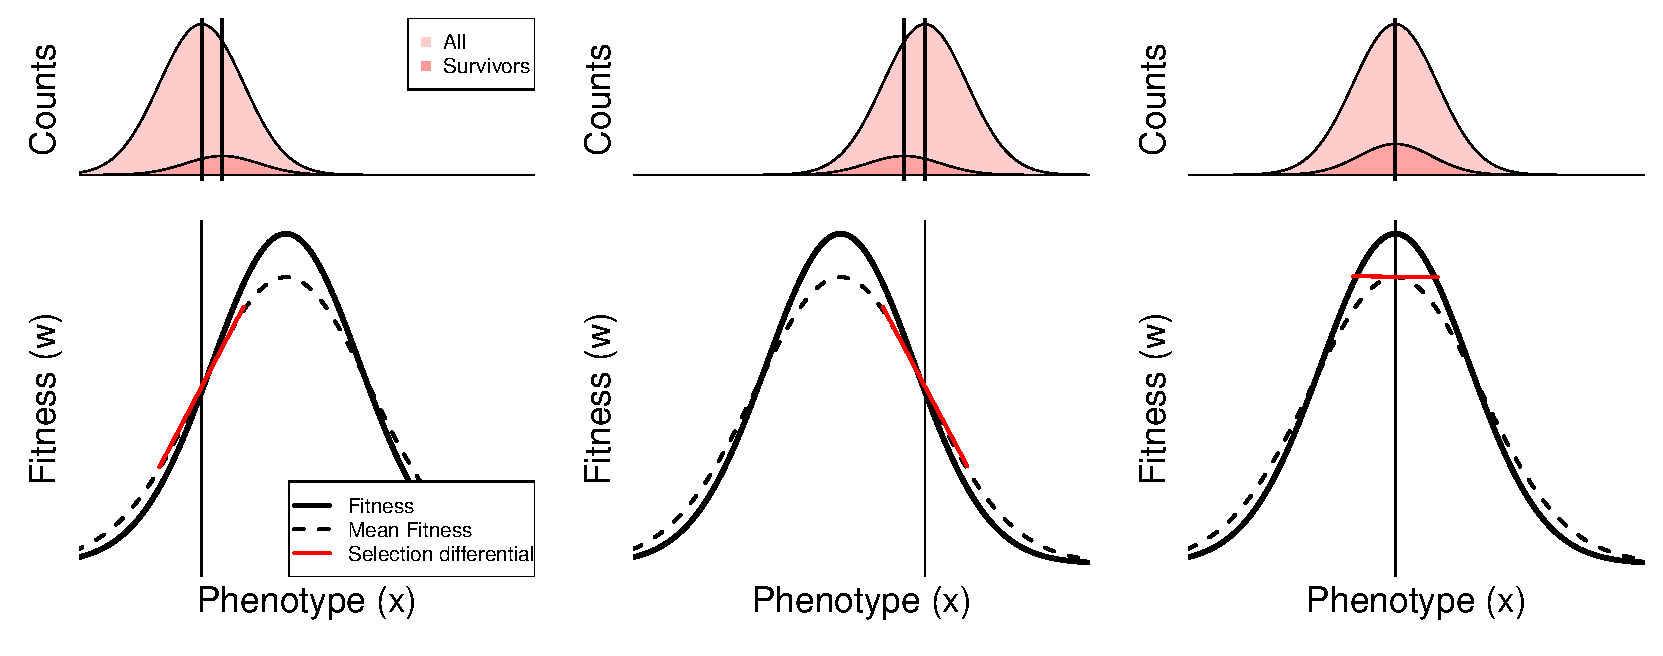
\includegraphics[width= 0.8 \textwidth]{figures/Response_to_sel/fitness_landscape_1D_w_wbar.pdf}
 \end{center}
 \caption{A population evolving on a (guassian) fitness surface. The
   bottom panel shows the expected individual fitness ($w()$) and mean
   fitess as a function of phenotype. The red line shows the best
   fitting linear approximation to the relationship between phenotype
   and individual fitness, eqn \eqref{fitness_regression}, whose slope is
   $\beta$. The top panel shows the distribution of the phenotype
   before and after selection. \gitcode{https://github.com/cooplab/popgen-notes/blob/master/Rcode/Quant_gen/fitness_landscape_1D_animated.R}.} \label{fig:fitness_landscape_1D_w_wbar}  
 \end{figure*}
 

What happens when it
reaches the top of a peak? Well at the top of a peak $ \nicefrac{\partial
  \wbar}{\partial \bar{x}}=0$, as it is a local maximum, and so
$R=0$. Assuming that the relationship between fitness and phenotype
stays constant, our population will stay at the top of the fitness
peak. This view of natural selection does not imply that the population
is evolving to the best possible state. Our population is just
marching up the hill of mean fitness (end panel Figure
\ref{fig:fitness_landscape_1D_w_wbar}). However, this peak isn't
necessarily the highest fitness peak but simply whichever peak was closest. So our population can become trapped
on a local, but not global peak of fitness (see, for example Figure \ref{fig:fitness_landscape_1D}).

% % \animategraphics[height=2.8in,autoplay,controls]{12}{/Users/gcoop/Downloads/latex_gif/animate_gall_}{0}{14}


One dramatic example documenting adaptive evolution to a new
fitness optimum is offered by a remarkable time-series of
stickleback evolution from a fossil lake-bed in Nevada \citep{bell2006inferring}. In this lake
the layers of sediment are laid down each year allowing a very detailed
time series with over five thousand fossils measured. The time-series
documents the evolution towards a new set of optimum phenotypes in the
fifteen thousand years after the initial invasion of the lake by a
heavily armoured stickleback species. In Figure \ref{fig:Stickleback_fossil_traj} the population mean number of
touching pterygiophores, the bones supporting the dorsal spines,
through the fossil record (Figure \ref{fig:Stickleback_fossil}). Note how quickly the species evolves toward
its new value, presumably a fitness optimum in their new environment, and the long subsequent time interval over which
the population mean phenotype fluctuates about its new value.

\begin{marginfigure}[3cm]
\begin{center}
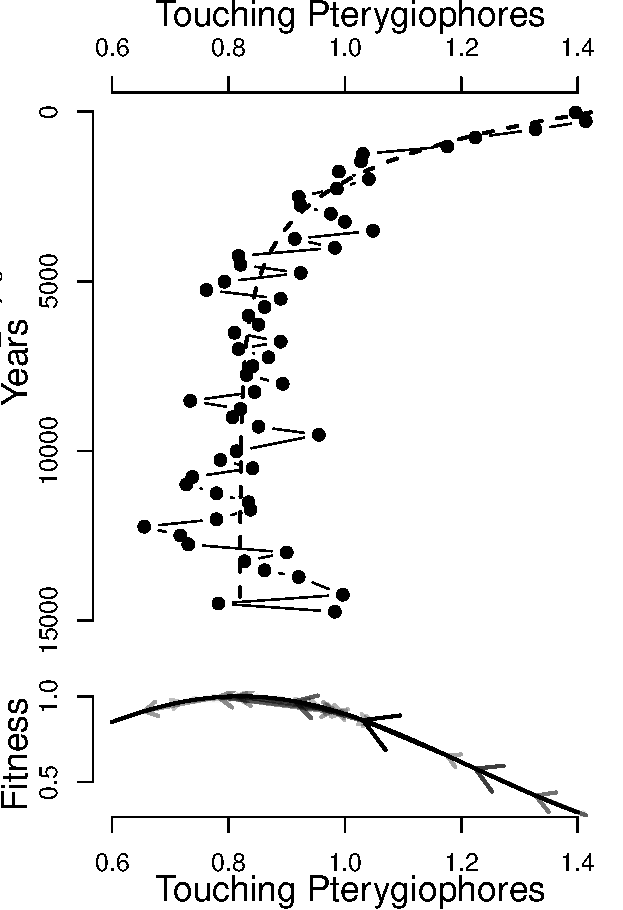
\includegraphics[width= \textwidth]{Journal_figs/Quant_gen/Stickleback_fossil_traj/Stickleback_fossil_traj.pdf}
\end{center}
\caption{{\bf Top)} A time series of stickleback phenotypic evolution from the
  fossil record. After a heavily armoured stickleback invades the lake
  it quickly evolves towards fewer touching pterygiophores (the bones
  supporting the dorsal spines).  Fossil measurements means are
  calculated in 250 year bins. {\bf Bottom)} How our population moves
  on the Inferred fitness landscape. The arrows show each move made by
  the population in the 250 intervals. Data from
  \citet{bell2006inferring} and \citet{hunt2008evolution}  \gitcode{https://github.com/cooplab/popgen-notes/blob/master/Journal_figs/Quant_gen/Stickleback_fossil_traj/Stickleback_traj.R} } \label{fig:Stickleback_fossil_traj}  
\end{marginfigure}

\citet{hunt2008evolution} fitted a model of a population adapting to a
fitness landscape, with a single peak, to these time-series data. Their fitted fitness
surface is shown in the lower panel of Figure \ref{fig:Stickleback_fossil_traj} . The arrows show the moves that the
population mean phenotype is making on this inferred fitness
surface. The population initially takes large steps up toward the peak
of this surface and subsequently fluctuates around the peak. Under the
interpretation that there is a single stationary peak these
fluctuations represent genetic drift randomly knocking the population
off its optimum, with selection acting to restore
the population towards this local optimum. \begin{marginfigure}
 \begin{center}
 \includegraphics[width= \textwidth]{illustration_images/Quant_gen/Fossil_stickleback/journal.pbio.1001466.g003.eps}
 \end{center}
 \caption{Fossil stickleback. Photo by Peter J. Park from \citet{losos2013evolutionary}, \PLOSccBY.} \label{fig:Stickleback_fossil}  
\end{marginfigure}

\paragraph{Issues with the interpretation of fitness landscapes.}
In practice, fitness landscapes may not be constant. The environment
may be constantly changing so our population is constantly forced to change to keep
up with the fitness peak. Indeed our environment may change so quickly
that our population cannot keep up with the peak. Our
population is still trying to increase its mean fitness, to `adapt', but
the landscape itself is evolving.\sidenote[][1cm]{In
the case of very rapid environmental change our population may slide
further and further away the peak, and as a consequence its mean fitness
decreases which may drive the population to extinction if our
population drops below $\wbar<1$ for long enough. The conditions for
extinction are an active area of research in the field of `Evolutionary rescue'.}
More generally, for our fitness landscape result (eqn \eqref{eqn:pheno_fitness_landscape}) to hold, and
for us to be able to talk of our population attempting to evolve to
higher mean fitness states,  we need the fitness of our phenotypes to be independent of the
frequency of other phenotypes in the population. (This independence allows us to
assume that the fitness of individuals is not a function of the mean
phenotype, as needed in eqn \eqref{eqn:proof_landscape}).  The
assumption of frequency independence may not hold when there is competition between individuals, e.g. for resources or
mates, as then the fitness of an individual depends on the strategies pursued
by other individuals in the populations.
%A classic example of this is
%the fact that sexual selection may drive our
%population towards pursing mate choice strategies that actively lower
%the mean fitness of the population. 
% \graham{Thinking of a marble
% rolling around in the bottom of a bowl
% You could think about the
% population phenotype as a marble rolling around  }

%\paragraph{Different populations potentially sit on top of different peaks in the fitness landscape}
 % https://journals.plos.org/plosbiology/article?id=10.1371/journal.pbio.1000529

 \subsection{Stabilizing and Disruptive selection}

Up to now we have just looked at directional selection, where
selection acts to change the mean phenotype. However, we
can also use quantitative genetic models to describe other modes of
selection, extending from effects on the population mean the next
natural step is to think about selection which acts on the
population variance. Selection might act more strongly against
individuals in the tails of the distribution, with those closer
to the mean phenotype having higher fitness, which lowers the
variance. Selection could also disfavour individuals close to the
population mean, with individuals with extreme phenotypes having
higher fitness, which acts to increase the variance of the population. 

Directional selection occurs because of the covariance
between our phenotype and fitness, eqn \eqref{S_covar}. Just as expressing directional selection as a covariance allowed us to
characterize directional selection as the linear relationship between
fitness and phenotype, $\beta$, we can summarize the variance
reducing selection by including a quadratic term in the regression of
fitness on phenotype
\begin{equation}
w_i \sim \beta x_i + \nicefrac{1}{2}  \gamma x_i^2  + \wbar \label{fitness_regression_stab}
\end{equation}
This $\gamma$, the coefficient of the quadratic term in our model, is the
quadratic selection gradient: the covariance of fitness and the squared
deviation from the phenotypic mean ($\mu_{BS}$), i.e.
\begin{equation}
\gamma = \frac{Cov\left(w(X), (X-\mu_{BS})^2 \right)}{V^2}
\end{equation}
Our $\gamma$ describes the curvature of the fitness surface around the
mean. \marginnote[-1.5cm]{Just like how $\beta$ could be interpreted
as the mean gradient of the fitness surface, our $\gamma$ is the
mean curvature of the fitness surface
  \begin{equation}
\gamma = \E \left[\nicefrac{\partial^2 w(x)}{\partial x^2}  \right] =
\int \nicefrac{\partial^2 w(x)}{\partial x^2} p(x) dx
\end{equation}
see Appendix Section \ref{section:calculus} for more on 2nd derivatives.
\graham{Need to straighten out issues with mean fitness vs fitness in
  these sections}
}
Values of $\gamma<0$  are consistent with stabilizing selection,
reducing the variance. While values of $\gamma>0$ are consistent with disruptive
selection, increasing the variance. \graham{add refs about this not being sufficient}

%To do this we can think about how selection acts 

% https://onlinelibrary.wiley.com/doi/pdf/10.1111/j.1469-1809.1951.tb02469.x

\begin{figure}
\begin{center}
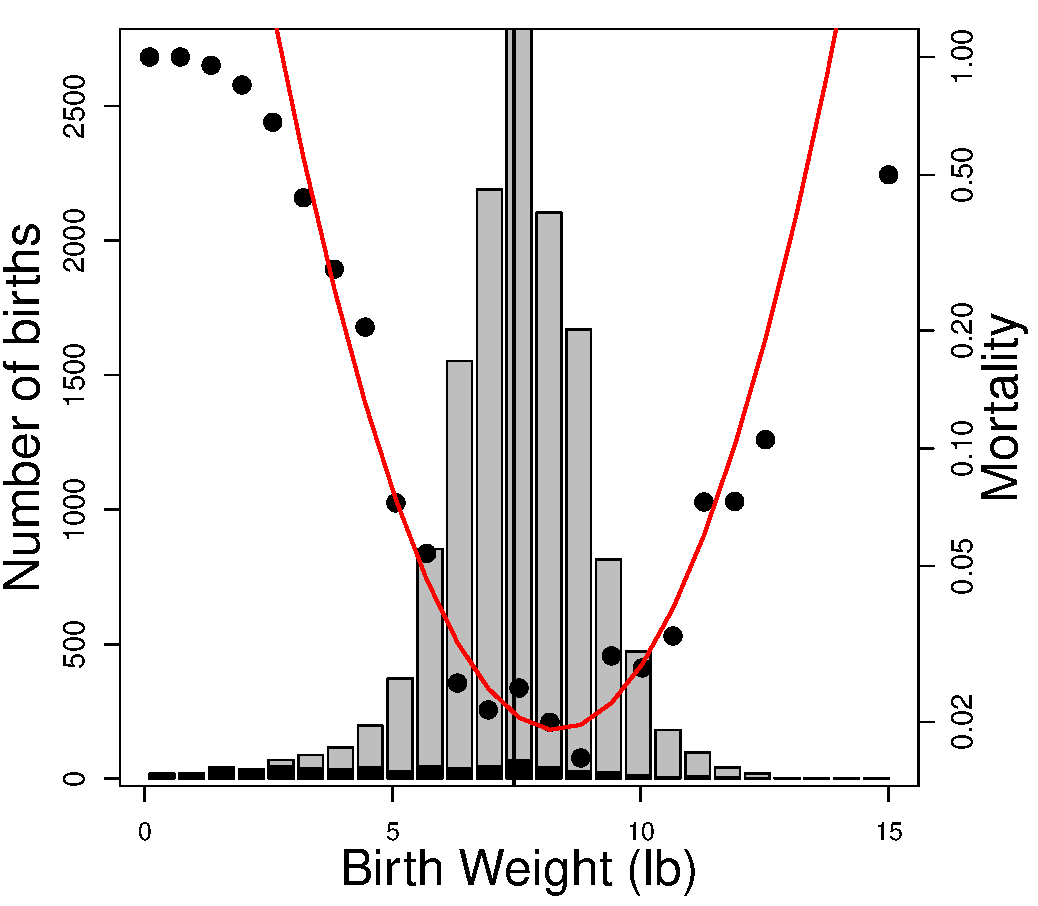
\includegraphics[width= 0.6 \textwidth]{Journal_figs/Quant_gen/birth_weight/Karn_Penrose_birth_weight.pdf}
\end{center}
\caption{Bars show the total number of births with different birth
  weights (left axis)  Dots show the mortality probability for different
  birth-weight bins (right axis), the red line shows a fitted
  quadratic model to mortality. Data from \citet{karn1951birth}
  Table 2, collapsing male and female births, \gitcode{https://github.com/cooplab/popgen-notes/blob/master/Journal_figs/Quant_gen/birth_weight/birth_weight_selection.R} } \label{fig:Birth_weight}  
\end{figure}

Under stabilizing selection the individuals with extreme phenotypes in
either tail have lower fitness, the result of which is to reduce the
phenotypic variance within a generation. A classic case of stabilizing selection
is birth weight in humans \citep{karn1951birth}. Mary Karn collected
data for nearly fourteen thousand pregnancies from 1935-46 for birth
weight and mortality. These data are replotted in Figure
\ref{fig:Birth_weight}. The variance of all births is $1.575$lb$^2$, while in live births this
was reduced to $1.26$lb$^2$, a 20\% reduction in variance due to
stabilizing selection. It is worth noting that this selection
pressure has been greatly reduced over the decades in societies with
access to good prenatal care \citep{ulizzi1992natural}.  %, a large effect of which has been to
%reduce the variance in birth weights due to better nutrition

%womb https://www.google.com/search?q=leonardo+da+vinci+baby&tbm=isch&source=iu&ictx=1&fir=pl1GYGee8iN0gM%253A%252CEdMTKcL8foK_hM%252C_&vet=1&usg=AI4_-kRCaAAUfKDX5AEtEm6lUZ5hjWMPlw&sa=X&ved=2ahUKEwjkluyapsniAhVWs54KHX7GBFsQ9QEwA3oECAMQCg#imgrc=W3ZPdyKQE9YkRM:&vet=1

\begin{marginfigure}
\begin{center}
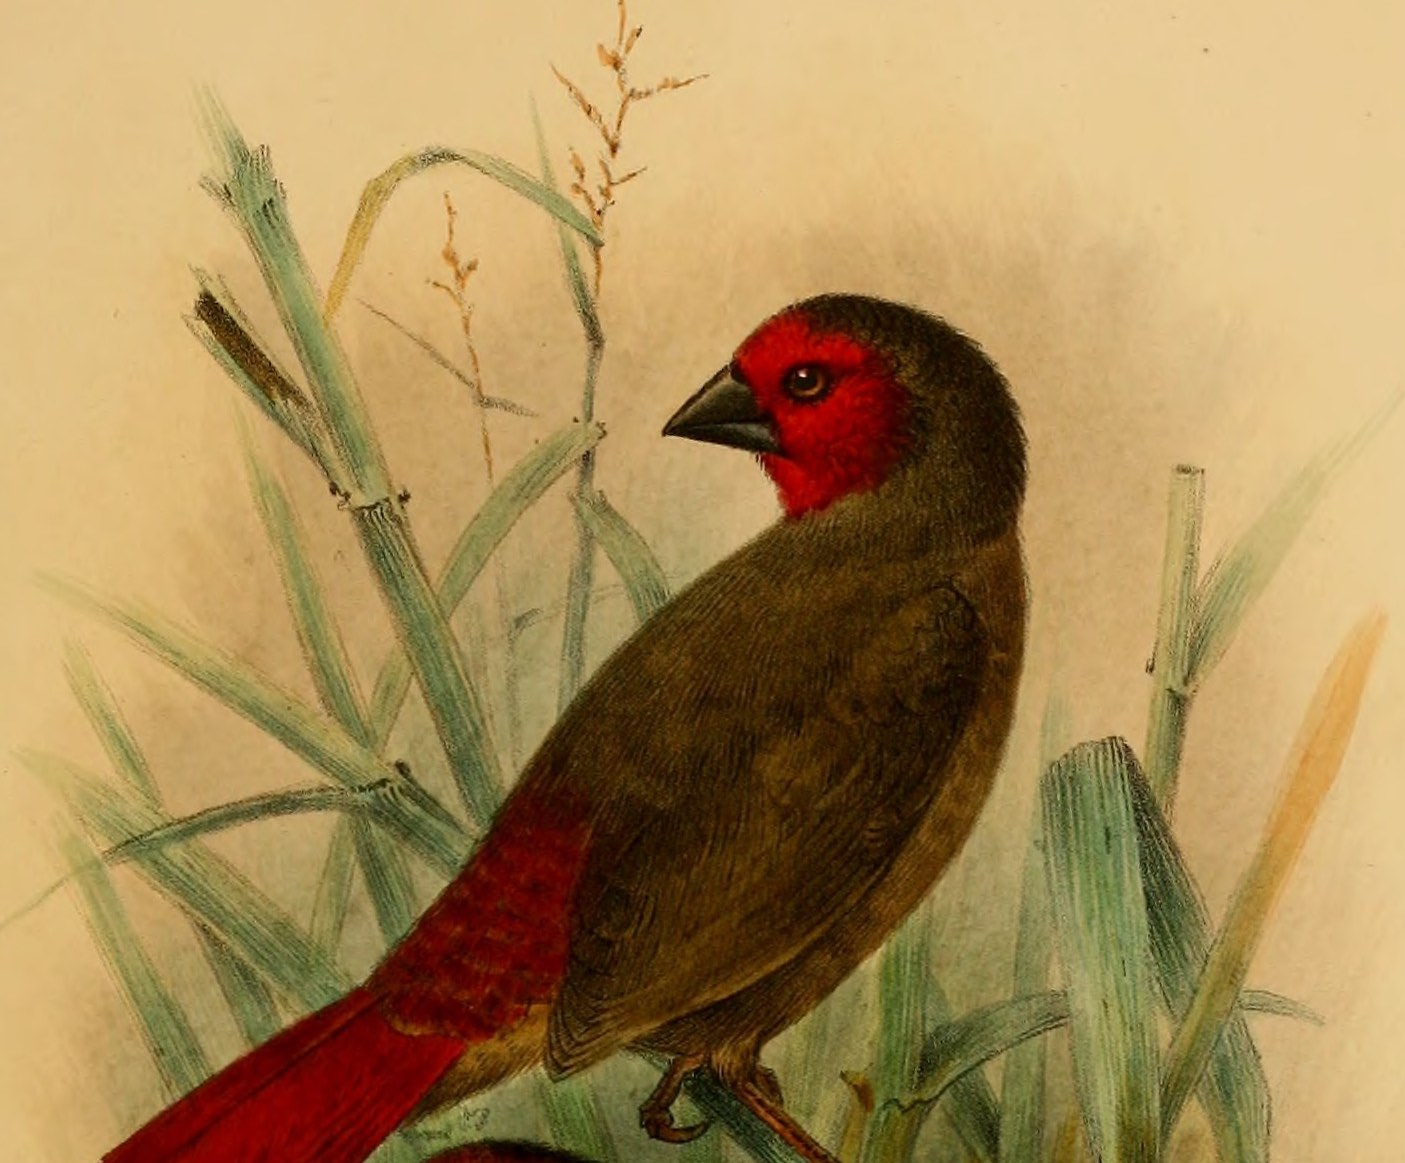
\includegraphics[width= \textwidth]{illustration_images/Quant_gen/Pyrenestes_seedcracker/Pyrenestes_minor.jpg}
\end{center}
\caption{Lesser seedcracker {\it Pyrenestes minor} a close relative of
  the Black-bellied seedcracker, whose beak is about the same size as
  the smallest Black-bellied individuals. \BHLNC{The birds of Africa, comprising all the species
    which occur in the Ethiopian region. (1986) Sclater, W. L Plate by  H. Gr{\"o}nvold}{https://archive.org/stream/birdsofafricacom41shel/birdsofafricacom41shel\#page/n306/mode/1up}{Smithsonian Libraries} }  
\end{marginfigure}
In Central Africa, Black-bellied seedcrackers ({\it
  Pyrenestes ostrinus}) show disruptive selection on a remarkable beak-size polymorphism (Figure \ref{Black_bellied_seedcrackers_beaks}).  The small-beaked individuals feed on
soft  seeds from one species of marsh sedge while the big-beaked
individuals feed on hard seeds from another sedge, which
requires ten times the force to crack. \citet{smith1993disruptive}
recorded the fates of hundreds of juveniles, and found that
individuals with intermediate beak sizes survived at much lower rates
(Figure \ref{Black_bellied_seedcrackers_beaks}) because they were not
well adapted to either seed resource.  Break length is subject to
disruptive selection, as can also be seen by the significant negative quadratic
term in the regression of survival probability on break length. The
variance of mandible length in the total sample of individuals was
$0.5$mm$^2$ in the survivors this variance increased by a factor of $2.5$ to $1.3$mm$^2$.  

\begin{figure}
\begin{center}
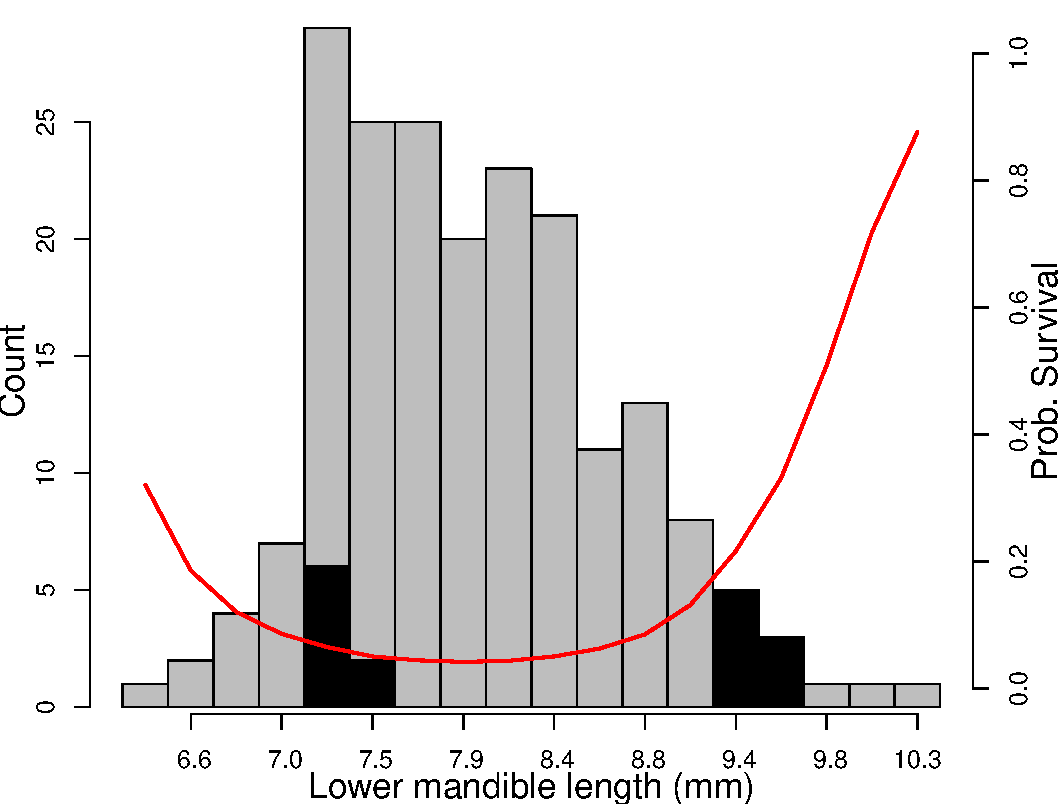
\includegraphics[width= \textwidth]{Journal_figs/Quant_gen/Smith_black_bellied_seed_cracker/Smith_black_bellied.pdf}
\end{center}
\caption{ {\bf Left} An illustration of the the remarkable variation
  in beak size within Black-bellied seedcrackers ({\it  P.
    ostrinus}). {\bf Right} A histogram of a beak size measurement in
  Black-bellied seedcrackers. All juveniles are shown in grey, while the
  black bars show the survivors. The red curve shows the best fitting
  linear and quadratic model to the probability of survival, fitted
  using a binomial generalized linear model with a logit link function.  
  \BHLNC{Left illustration from: Size variation in {\it Pyrenestes} by
    Chapin J.P. in the Bulletin of the
    American Museum of Natural History (Vol. XLIX
    1923)}{https://archive.org/stream/bulletinofameric49alleuoft/\#page/417/mode/1up}{Toronto
    Library}   } \label{Black_bellied_seedcrackers_beaks}
\end{figure}


To illustrate how directional selection and quadratic terms play off
during adaptation, lets consider the goldenrod gall fly ({\it Eurosta solidaginis}), aka the goldenrod
ball gallmaker. See Figure \ref{gall_size_stab}. As it's wonderful name
implies this insect lays its eggs in Goldenrod plants, and the larvae
release chemicals forcing the plant to form a gall that forms a home
for the larvae as they develop. While this seems like a pretty sweet
deal for the larvae, it is not without its perils. \begin{marginfigure}[2cm]
\begin{center}
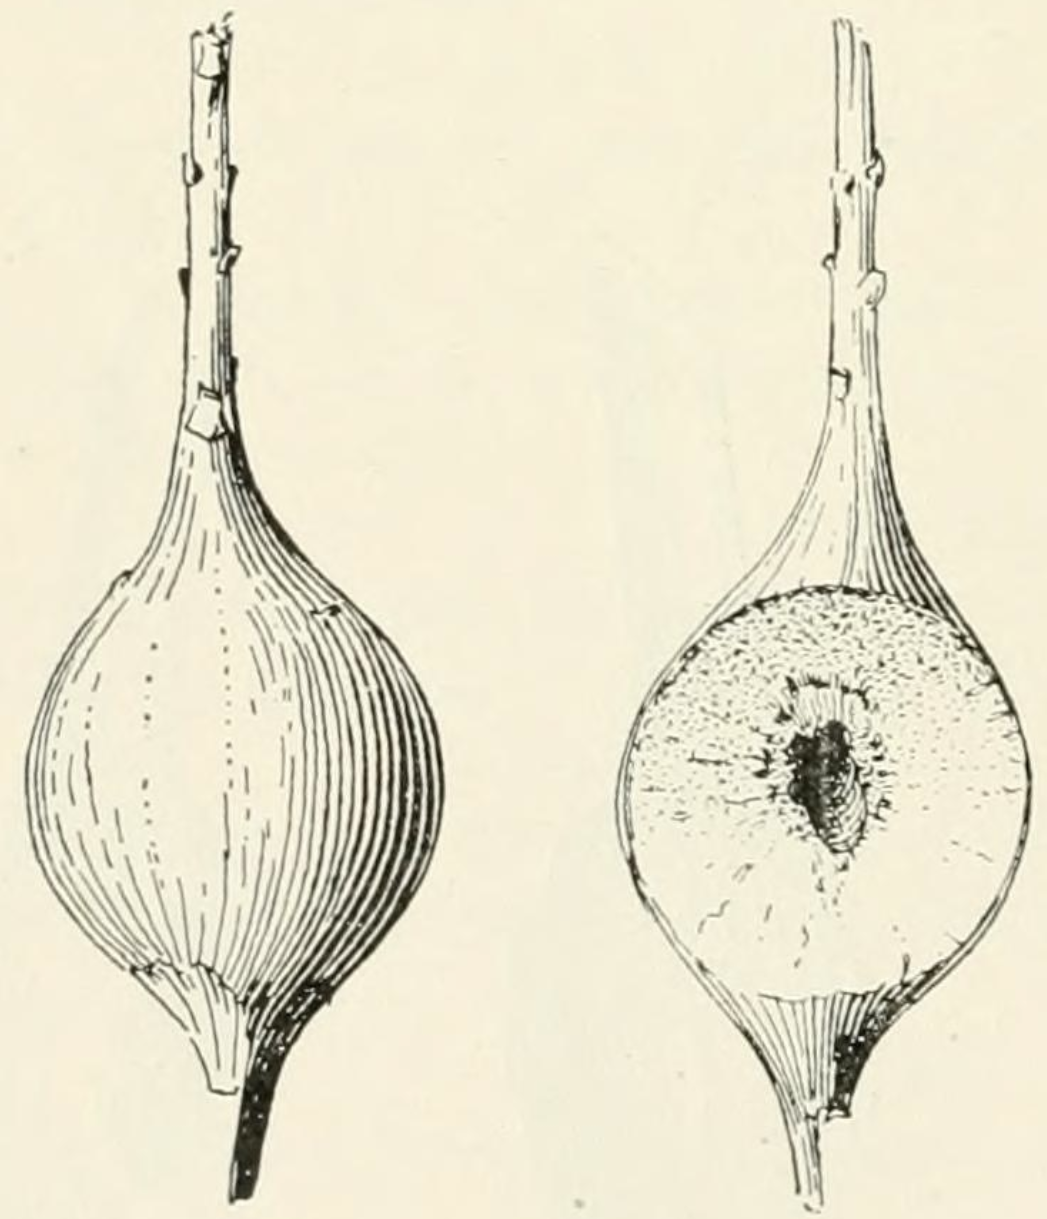
\includegraphics[width= 0.7 \textwidth]{illustration_images/Quant_gen/goldenrod_ball_gall_maker/goldenrod_ball_gall_maker.png}
\end{center}
\caption{The gall formed by the goldenrod
ball gallmaker ({\it Eurosta solidaginis}) in a goldenrod plant. The
one on the right is cut to show a partial cross-section. \BHLNC{Annual report of the New York State Museum (1917)}{https://archive.org/stream/annualreport71newy/\#page/196/mode/1upp}{The LuEsther T Mertz Library, the New York Botanical Garden} }  
\end{marginfigure}
When the small, ball galls fall risk of parasitism from parasitoid
wasps. When all the ball galls are small in the population selection drives strong positive directional selection on
gall size, with little stabilizing selection. Notice in the left panel
of Figure \ref{gall_size_stab} the good
agreement between the linear selection gradient and the fit including
a linear and quadratic term. However, bigger galls fall under the pall of predation from downy
woodpeckers and black-capped chickadees, who seek out the tasty
larvae. Thus intermediate size galls are favoured, a fitness peak that
the population quickly reaches. Once on this peak,
as shown in the right panel of Figure \ref{gall_size_stab} there is no directional selection, i.e. no linear slope, but there
is strong stabilizing selection, i.e. a quadratic term. Thus the
population will be maintained at this fitness peak indefinitely if the
environment remains unchanged.

\begin{figure}
\begin{center}
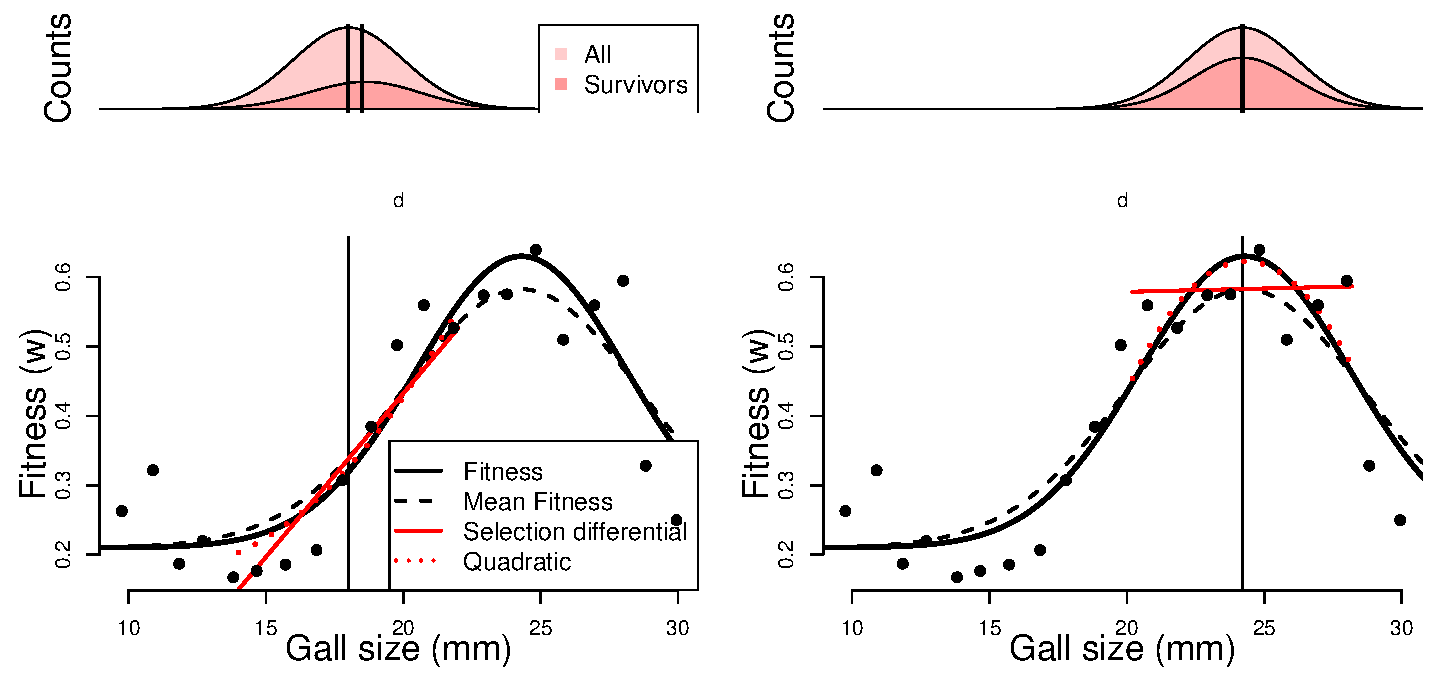
\includegraphics[width= \textwidth]{Journal_figs/Quant_gen/Weis_Gorman_gall_size_stablizing_sel/gall_size.pdf}
\end{center}
\caption[][4cm]{Fitness surface for gall diameter in goldenrod
ball gallmakers. The dots are the measured survival probabilities of
bins of different sized galls.The solid line is a fitted individual fitness
  surface ($w(~)$). Dotted line is $\wbar$ plotted as a function of
  the population mean assuming a normal distribution with a standard
  deviation of $2$mm. Data from \citet{weis1990measuring}, \gitcode{https://github.com/cooplab/popgen-notes/blob/master/Journal_figs/Quant_gen/Weis_Gorman_gall_size_stablizing_sel/gall_size_fitness_landscape.R}} \label{gall_size_stab}
\end{figure}


%%% selection on gall size https://sci-hub.tw/https://onlinelibrary.wiley.com/doi/abs/10.1111/j.1558-5646.1990.tb03807.x
% https://www.flickr.com/photos/internetarchivebookimages/18429735991/
%https://archive.org/stream/annualreport71newy/#page/196/mode/1up


%black beelied seed cracker
%https://sci-hub.tw/https://www.nature.com/articles/363618a0
%https://www.flickr.com/photos/internetarchivebookimages/20416920856/in/photolist-otagrj-xVVxst-wRSxF1-x7b4fQ-x9uxzB
%https://www.flickr.com/photos/internetarchivebookimages/14755609045/
 
% Cross bill https://www.google.com/search?q=loxia+curvirostra+biodiversity+heritage+library&source=lnms&tbm=isch&sa=X&ved=0ahUKEwjItfbRm87iAhUyMn0KHZDNDlIQ_AUIECgB&biw=1440&bih=726#imgrc=cfi-GvhZRX1zxM:
% https://sci-hub.tw/https://www.jstor.org/stable/2937103?seq=1#metadata_info_tab_contents


%file:///Users/gcoop/Downloads/calsbeek2008.pdf  disruptive selection
%on leg length in anoles
 
